% !TEX root = coatlioan.tex

\chapter{The Huitzi Imager}

The Huitzi imager was installed on the COATLI telescope in October 2021. The imager is named for the mexica god \href{https://en.wikipedia.org/wiki/Huītzilōpōchtli}{Huītzilōpōchtli}, the son of the goddess Coatlicue.

\section{Introduction}

The Huitzi imager has an Andor iXon electron-multiplying CCD detector with $1024\times1024$ pixels with a pixel scale of 0.68 arcsec and a field of 11.6 arcmin. The detector can be read through either a conventional amplifier or the electron-multiplying amplifier at a variety of speeds.

The image also has Finger Lakes Instruments CFW-1-8 filter wheel for eight 25 mm diameter filters. At the time of writing, the following filters are installed:
\begin{itemize}
    \item Pan-STARRS $griz$;
    \item 470/10, 640/10 continuum;
    \item 656/3 H$\alpha$; and
    \item a dark filter.
\end{itemize}

\begin{figure*}
\begin{center}
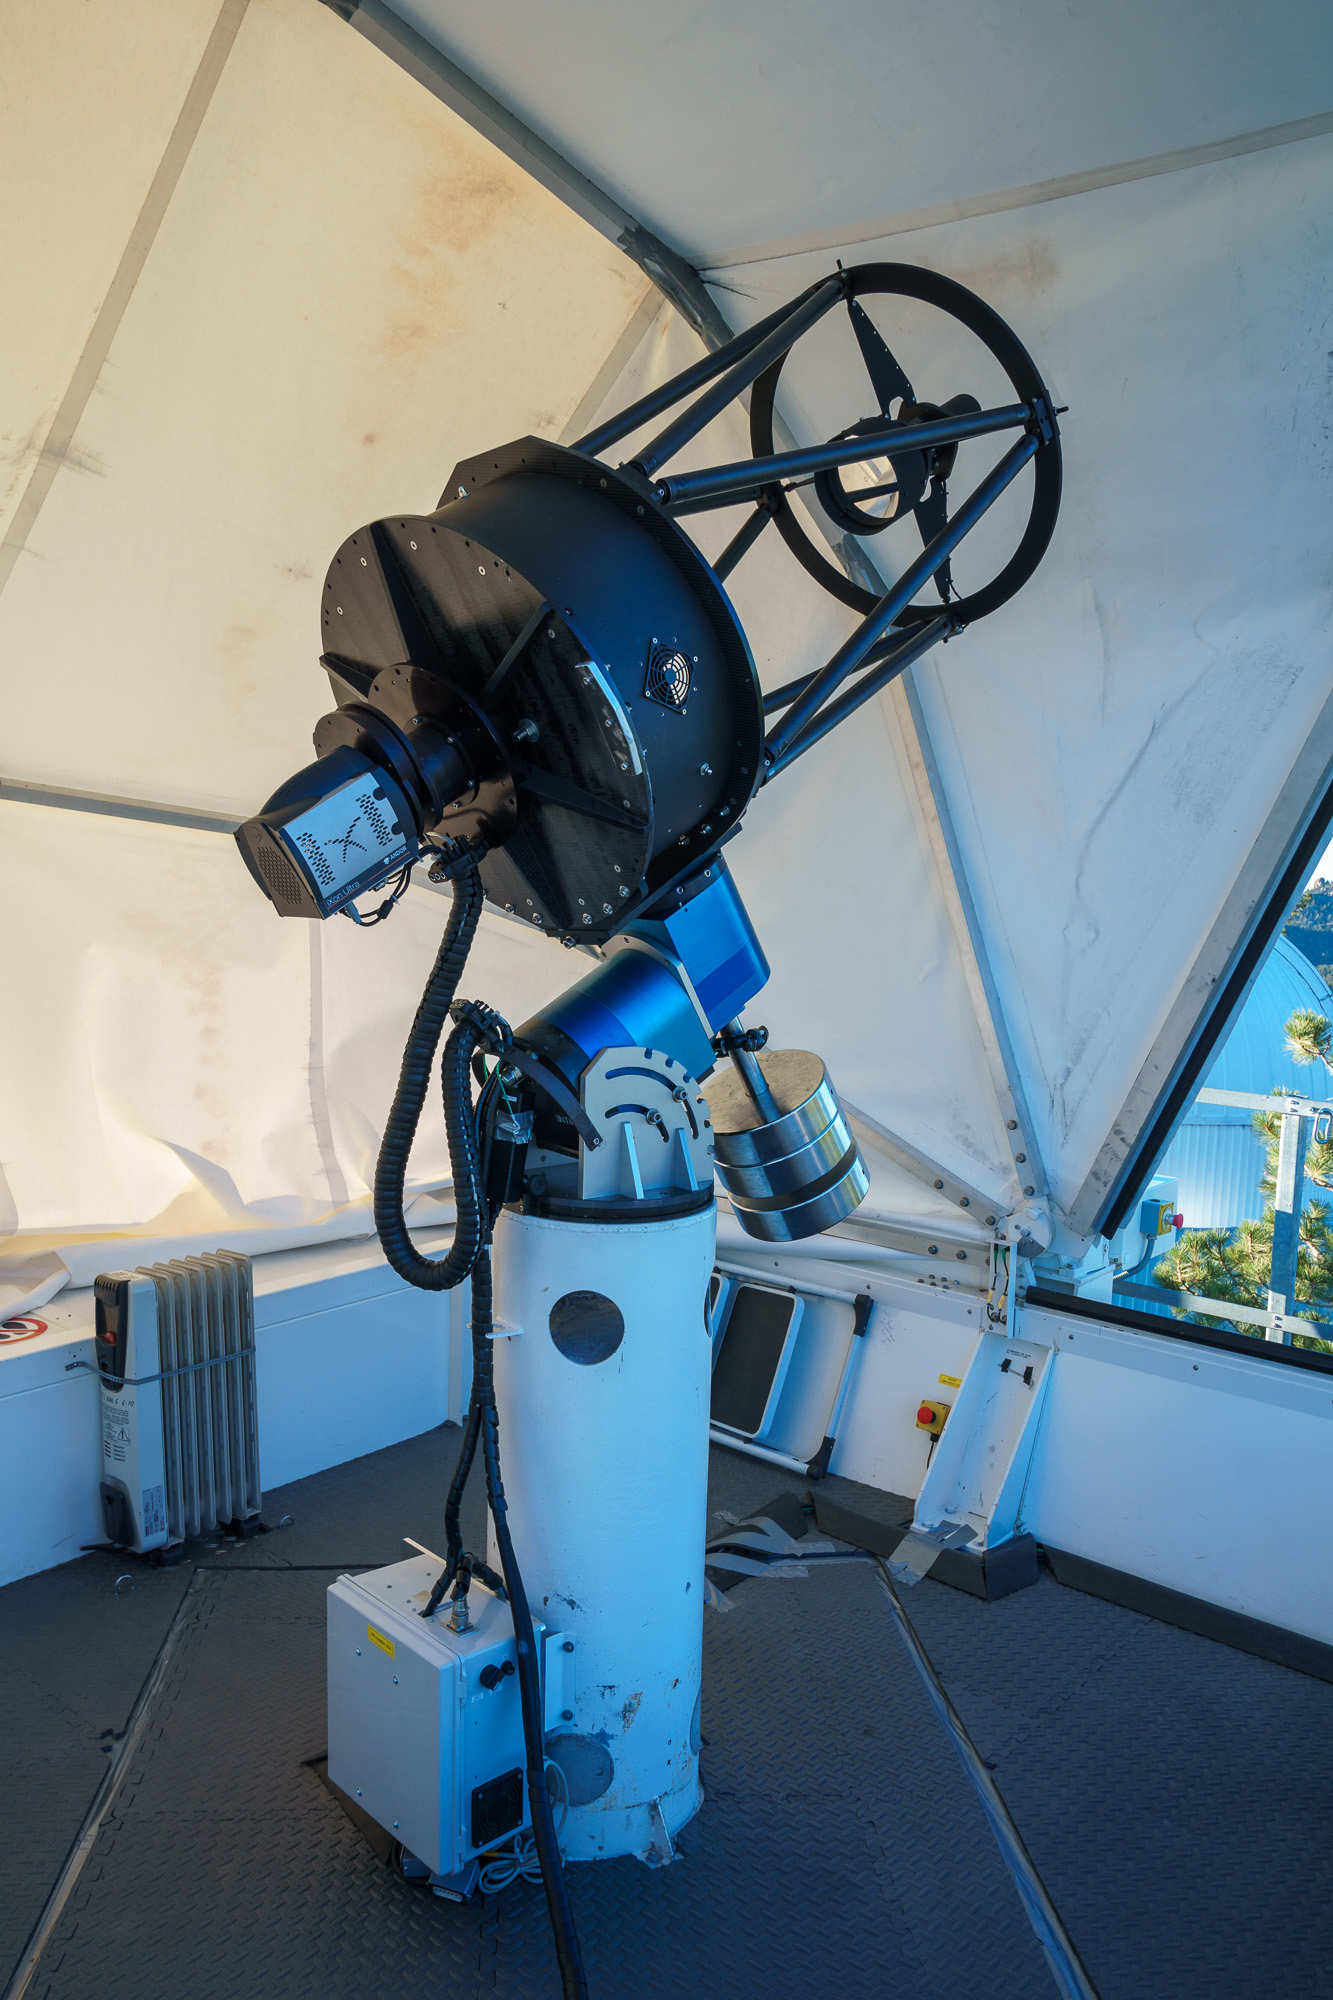
\includegraphics[width=0.45\linewidth]{figures/huitzi-hardware.jpg}
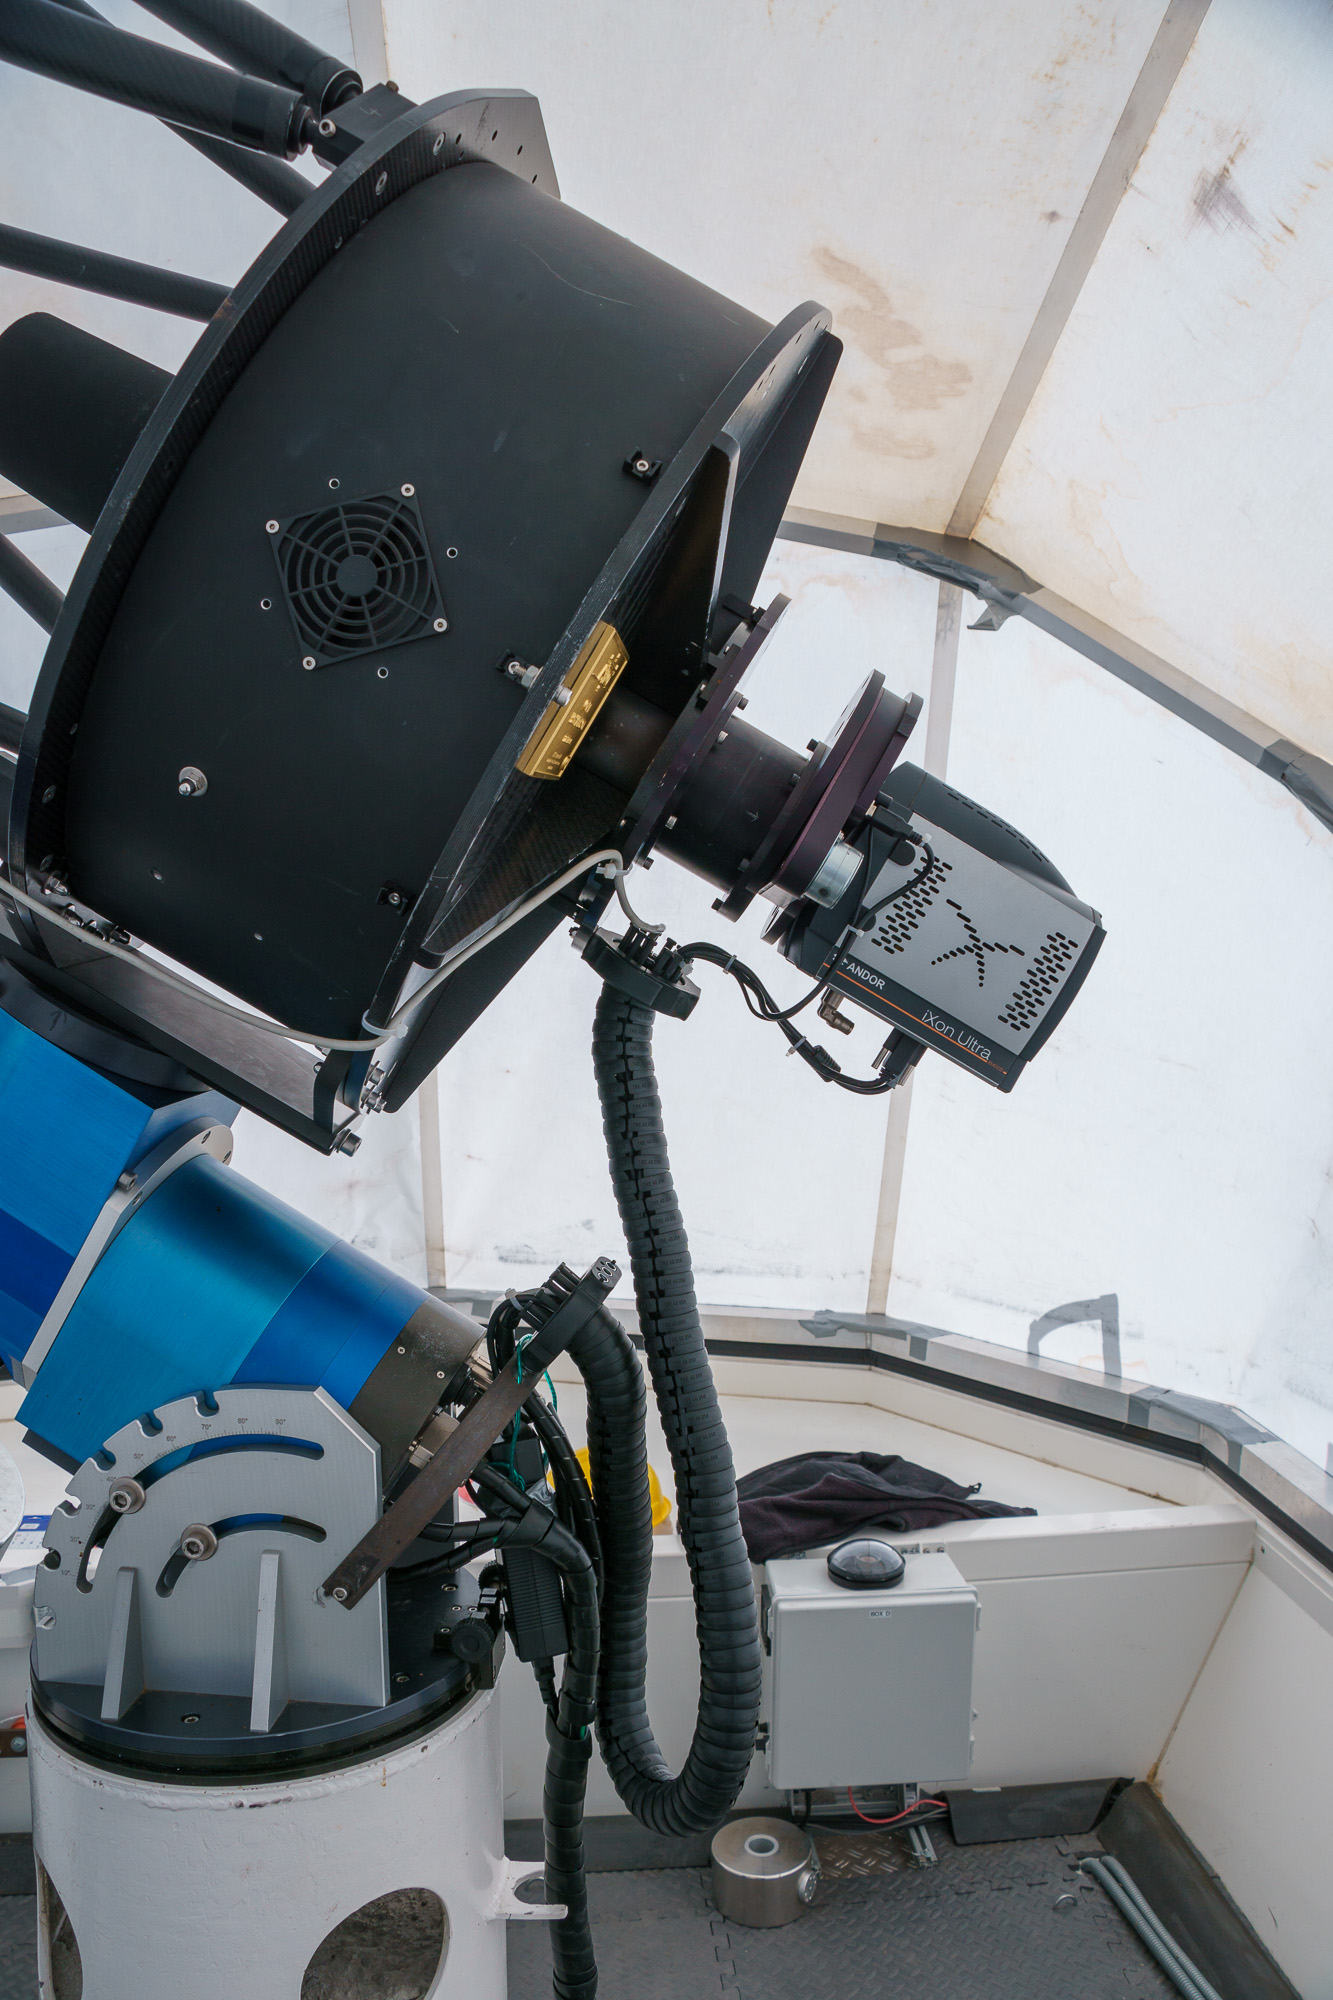
\includegraphics[width=0.45\linewidth]{figures/huitzi-hardware-telescope.jpg}
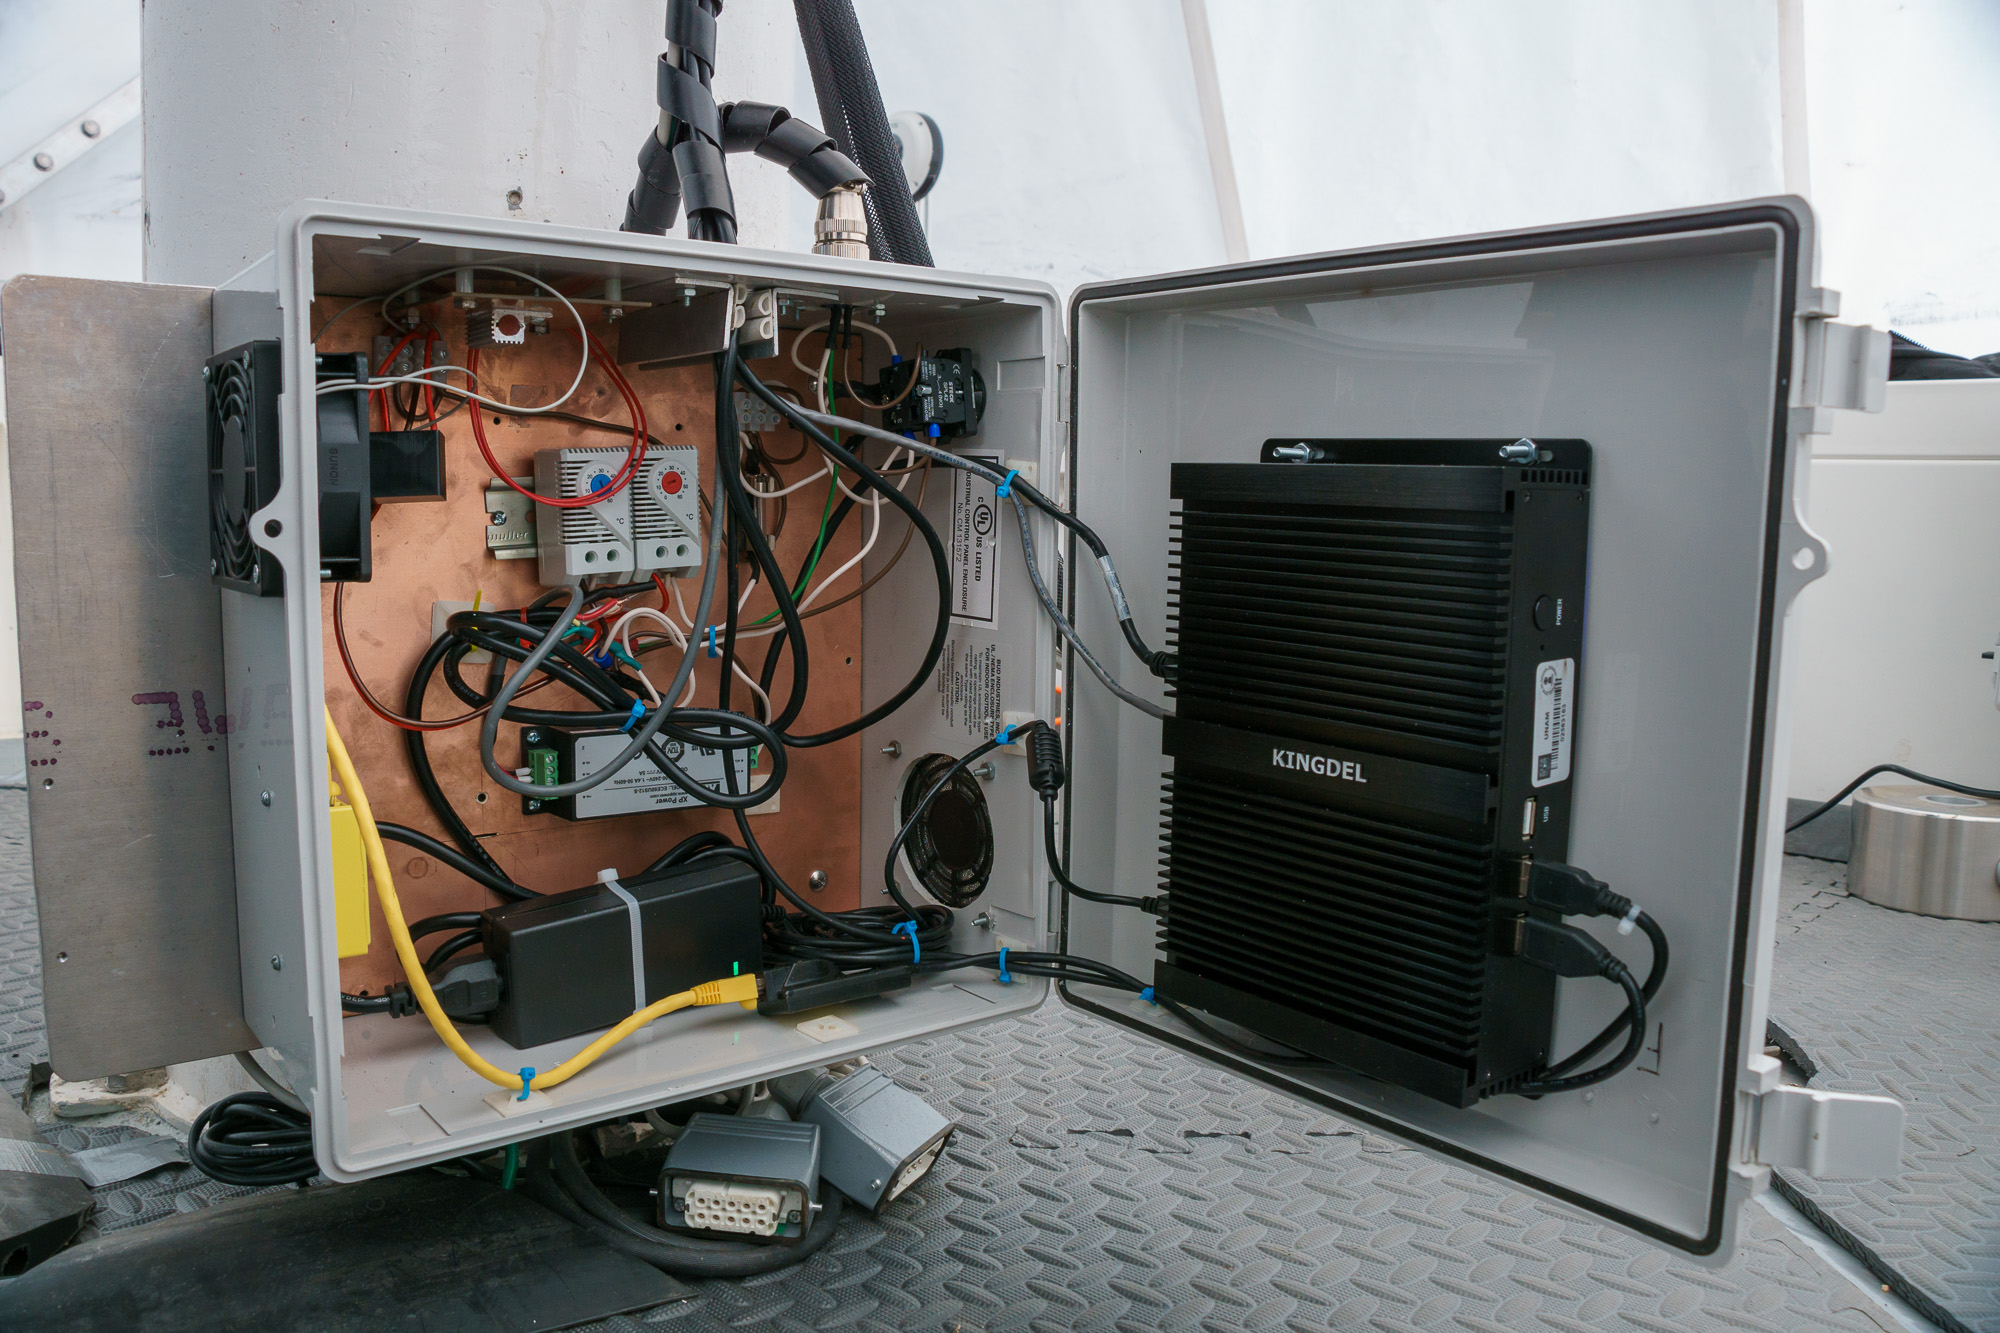
\includegraphics[width=0.675\linewidth]{figures/huitzi-hardware-electronics.jpg}
\end{center}
\caption{The Huitzi hardware. On the telescope the principal components are the Andor iXon detector and FLI filter wheel. The control electronics are located in the box mounted on the south side of the pillar. The cables pass up onto the telescope through an Igus Triflex chain.}
\label{figure:huitzi-hardware}
\end{figure*}

The hardware of the Huitzi instrument is shown in Figure~\ref{figure:huitzi-hardware}. On the telescope the principal components are the Andor iXon detector and FLI filter wheel. The control electronics are located in the box mounted on the south side of the pillar. The cables pass up onto the telescope through an Igus Triflex chain. The mechanical hardware is adapted from the previous interim imager (see Appendix~\ref{appendix:interim-imager}).

\section{Detector}

The detector unit is an Andor iXon Ultra 888 with an e2v CCD201-20 electron-multiplying CCD detector. The detector was acquired in 2014 and originally intended to be the tilt sensor for the planned two-channel imager.

\subsection{Format, Scale, and Field}

The detector has $1024\times1024$ pixels each $13\times13$ {\micron} square. 

The detector gives a pixel scale of 0.68 arcsec and a field of 11.6 arcmin. 

\begin{figure}
\begin{center}
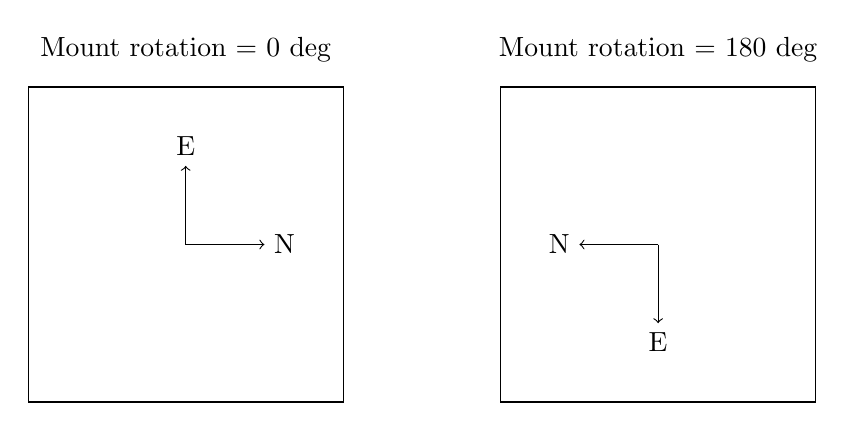
\begin{tikzpicture}
\begin{scope}[xshift=-3cm]
\draw (-2,-2) -- (+2,-2) -- (+2,+2) -- (-2,+2) -- cycle;
\draw (0,2.2) node [anchor=south] {Mount rotation = 0 deg};
\draw[->] (0,0) -- (1,0) node [anchor=west] {N};
\draw[->] (0,0) -- (0,1) node [anchor=south] {E};
\end{scope}
\begin{scope}[xshift=3cm]
\draw (-2,-2) -- (+2,-2) -- (+2,+2) -- (-2,+2) -- cycle;
\draw (0,2.2) node [anchor=south] {Mount rotation = 180 deg};
\draw[->] (0,0) -- (-1,0) node [anchor=east] {N};
\draw[->] (0,0) -- (0,-1) node [anchor=north] {E};
\end{scope}
\end{tikzpicture}
\end{center}
\caption{The orientation of the detector on the sky according to the mount rotation. The pixel origin is in the lower left.}
\label{figure:detector-orientation}
\end{figure}

The orientation of the field on the sky depends on the mount rotation (given by the values of the \verb|SMTMRO| and \verb|EMTMRO| keywords in the header), and is shown in Figure~\ref{figure:detector-orientation}. However, the pipeline reduction rotates all images to the conventional orientation with north up and east left.

\subsection{Quantum Efficiency}

The detector has standard silicon and the e2v midband coating (which in Andor's terminology makes it a “BV” device). The nominal quantum efficiency is shown in Figure~\ref{figure:detector-quantum-efficiency}. The detector has excellent efficiency from 500 to 800 nm.

\begin{figure}
\begin{center}
\begin{tikzpicture}
\small
\begin{axis}[
   xmin=300,
   xmax=1100,
   xlabel={$\lambda$ (nm)},
   xticklabel style={
     /pgf/number format/precision=0,
     /pgf/number format/fixed,
     /pgf/number format/fixed zerofill
   },
   minor x tick num=3,
   ymin=0,
   ymax=1,
   minor y tick num=3,
   ylabel={$\eta$},
   legend style={
     cells={anchor=west},
     legend pos=north east,
   },
]
\addplot [black] table [x=lam, y=Q, col sep=comma] {figures/huitzi-detector-efficiency.csv};
\end{axis}
\end{tikzpicture}
\end{center}
\caption{The nominal quantum efficiency $\eta$ of the Huitzi detector.}
\label{figure:detector-quantum-efficiency}
\end{figure}


\subsection{Readout Architecture}

The detector can be read using either a conventional signal chain (at 100 kHz or 1 MHz) or an EM signal chain (at 1, 10, 20, or 30 MHz). Both chains have two gains and the EM gain can be set to up to 1000. 

Although the conventional and EM amplifiers clock the serial register in different directions, the control software flips each row in conventional data so that physical pixels have the same logical position in the FITS files.

The detector is used in frame-transfer mode without a mechanical shutter (see \S\ref{section:shutter}). At the end of an exposure, the charge is rapidly clocked into from the light-sensitive image section to the shielded store section. The change can then be read. In EM mode, the next exposure can then start immediately.

With the normal vertical-shift frequency of 4.33 MHz, the frame transfer takes about 4.5 ms. This leads to some trailing above and below bright stars.

The read-out architecture has several parameters, which are encoded in the value of the \verb|READMODE| header keyword. The value is a string of the form $A$-$B$-$C$-$D$-$E$-$F$-$G$ in which $A$ to $G$ are non-negative integers with the following meanings:

\begin{itemize}
\item[$A$] The ADC channel index. This is always 0 since the detector only has one ADC channel.
\item[$B$] The amplifier index. This is 0 for the EM amplifier and 1 for the conventional amplifier.
\item[$C$] The vertical shift speed index. For both amplifiers, 0 is 0.60 MHz, 1 is 1.13 MHz, 2 is 2.20 MHz, and 3 is 4.33 MHz. 
\item[$D$] The horizontal shift speed index. For the EM amplifier, 0 is 30 MHz, 1 is 20 MHz, 2 is 10 MHz, and 3 is 1 MHz. For the conventional amplifier, 0 is 1 MHz and 1 is 100 kHz.
\item[$E$] The gain index. For both amplifiers, 0 is low gain (more electrons per ADU) and 1 is high gain (fewer electrons per ADU).
\item[$F$] The nominal EM gain. This is ignored when the conventional amplifier is used. For the EM amplifier, it can be between 1 and 1000.
\item[$G$] The software gain. After the data are read, each ADU signal is divided by the software gain to reduce white noise in the low-order bits (see \href{https://ui.adsabs.harvard.edu/abs/2002RMxAA..38..233W/abstract}{Watson 2002, RMAA, 38, 233}).
\end{itemize}

Fortunately, there is little need to use these values directly, since aliases are defined for common modes. They are shown in Table~\ref{table:read-mode-aliases}.

\begin{table}
\caption{Read-Mode Aliases}
\label{table:read-mode-aliases}
\begin{center}
\begin{tabular}{lll}
\hline
Alias&Mode\\
\hline
 initial&default\\
 default&em-30MHz\\
 conventionaldefault&1MHz\\
 fastguidingdefault&em-30MHz\\
 1MHz&1MHz-low\\
 em-10MHz&em-10MHz-low\\
 em-20MHz&em-20MHz-low\\
 em-30MHz&em-30MHz-low\\
 1MHz-low&0-1-3-0-0-1-1\\
 1MHz-high&0-1-3-0-1-1-2\\
 em-10MHz-low&0-0-3-2-0-250-2\\
 em-10MHz-high&0-0-3-2-1-160-4\\
 em-20MHz-low&0-0-3-1-0-500-4\\
 em-20MHz-high&0-0-3-1-1-320-8\\
 em-30MHz-low&0-0-3-0-0-1000-8\\
 em-30MHz-high&0-0-3-0-1-640-16\\
 \hline
\end{tabular}
\end{center}
\end{table}

\subsection{Shutter and Dark Filter}

\label{section:shutter}

The detector has a conventional mechanical iris shutter, but we do not use it.

We originally attempted to use the mechanical shutter for conventional CCD modes and the frame-transfer capability for EM modes. However, we found that the shutter sometimes failed to open or failed to open completely. We suspect that at the colder temperatures at night, the power supply does not provide sufficient voltage to open the shutter. 

Therefore, we now leave the shutter open permanently and use the frame-transfer capability in both conventional and EM modes. As noted above, with the normal vertical-shift frequency, the frame transfer takes about 4.5 ms.

To take bias and dark images, we have installed a “dark” filter (an opaque cylinder of black Delrin 25 mm in diameter and 5 mm thick) in the filter wheel. Despite this, light leaks in the filter wheel mean that we need to take biases and darks at night.

\begin{table}
    \centering
    \begin{tabular}{lcccc}
    \hline
    Mode Name&1MHz-0&em-10MHz-0&em-20MHz-0&em-30MHz-0\\
    \hline
    Amplifier&Conventional&EM&EM&EM\\
    Horizontal Speed&1 MHz&10 MHz&20 MHz&30 MHz\\
    Software Gain&1&2&4&8\\
    ADC Range (DN)&64k&32k&16k&8k\\
    Gain ($e^-$/DN)&3.3&41&78&117\\
    Read Noise (DN)&2.1&2.6&1.9&1.7\\
    Read Noise ($e^-$)&7&105&145&204\\
    Bias Level (DN)&500&242&123&62\\
    Linear Limit ($e^-$)&&400k&400k&400k\\
    Saturation (DN)&58k&32k&16k&8k\\
    Saturation ($e^-$)&190k&1300k&1250k&940k\\
    Linearity ($e^-$)&&400k&400k&400k\\
    Linearity (DN)&&9700&5100&3400\\
    Dynamic Range (bits)&&11.9&11.4&10.9\\
    \hline
    \end{tabular}
    \caption{Detector Characteristics with the Low Preamplifier Gain}
    \label{table:detector-characteristics-low-gain}
\end{table}

\begin{table}
    \centering
    \begin{tabular}{lcccc}
    \hline
    Mode Name&1MHz-1&em-10MHz-1&em-20MHz-1&em-30MHz-1\\
    \hline
    Amplifier&Conventional&EM&EM&EM\\
    Horizontal Speed&1 MHz&10 MHz&20 MHz&30 MHz\\
    Software Gain&2&4&8&16\\
    ADC Range (DN)&32k&16k&8k&4k\\
    Gain ($e^-$/DN)&1.6&21&45&70\phantom{0}\\
    Read Noise (DN)&2.9&2.7&2.4&1.6\\
    Read Noise ($e^-$)&5&56&108&115\\
    Bias Level (DN)&250&119&62&31\\
    Saturation (DN)&22k&\\
    Saturation ($e^-$)&35k&\\
    Linearity ($e^-$)&&400k&400k&400k\\
    Linearity (DN)&&19000&8900&5700\\
    Dynamic Range (bits)&&12.8&11.9&11.8\\
    \hline
    \end{tabular}
    \caption{Detector Characteristics with the High Preamplifier Gain}
    \label{table:detector-characteristics-high-gain}
\end{table}

\section{Filter Wheel}

The slots are filled as follows:
    \begin{enumerate}
        \item[0:] $g$
        \item[1:] $r$
        \item[2:] $i$
        \item[3:] $z$
        \item[4:] 470/10
        \item[5:] dark
        \item[6:] 640/10
        \item[7:] 656/3
    \end{enumerate}
    
\section{Filters}


\section{Mounting Hardware}

\section{Control Hardware}

\section{Control Software}

\section{Calibration Data}

\subsection{Biases and Darks}

\subsection{Flats}

\subsection{Gain and Read Noise}

The control system does not automatically take data for calibrating the gain and read-noise, but there are blocks that can be executed manually either in evening or morning twilight. 

For best results, do this procedure either at the start of evening civil twilight or the start of morning nautical twilight.

The procedure is:

\begin{itemize}
\item Make sure the telescope is closed:
\begin{verbatim}
tcs request supervisor close
\end{verbatim}
\item Unpark the telescope and cool the instrument:
\begin{verbatim}
tcs request telescope unpark
tcs request instrument open
\end{verbatim}
\item Wait for the detector to cool to the operating temperature. Then run the morning or evening block, as appropriate:
\begin{verbatim}
tcs request executor execute block \
  /usr/local/var/tcs/blocks/0013-signal-chain-morning.json
tcs request executor execute block \
  /usr/local/var/tcs/blocks/0013-signal-chain-evening.json
\end{verbatim}
The difference between the blocks is that in the morning the block takes biases and then flats, whereas in the evening it takes flats and then biases.
\item
One the block has finished, close the telescope again by running:
\begin{verbatim}
tcs request executor close
\end{verbatim}
\end{itemize}

For these data:
\begin{itemize}
\item The program identifier is 0013. 
\item The block identifier is 0 for the morning and 1 for the evening. 
\item Visit 0 is for readmode “1MHz-low” and visit 1 is for readmode “1MHz-high”.
\end{itemize}

In each readmode, the block takes 10 biases and attempts to obtain 10 flats with levels suitable for determining the gain. These flats will normally be the last 10 flats, as the block waits for the signal in the flat to be in a suitable range.

The dome lights should not be switched on during this process. If they are, then the biases will be contaminated with light, since the dark filter has light leaks, and the flats will be saturated. Note that sometimes the technical staff switch the lights on in the morning to check that the enclosures have closed, so you should warn them in the chat that you are taking calibration data and that they should not do this.

\section{Maintenance Procedures}

\subsection{Dismounting and Mounting the Instrument}
\label{section:huitzi-dismounting-and-mounting}

\subsubsection{Requirements}

You will need:

\begin{itemize}
    \item Two persons.
    \item The key to the shed (see \S\ref{figure:buildings-shed-key}).
    \item 4 mm and 2 mm hex keys
    \item 5/16 inch hex key.
\end{itemize}

\subsubsection{Dismounting the Imager}

\begin{figure*}
\begin{center}
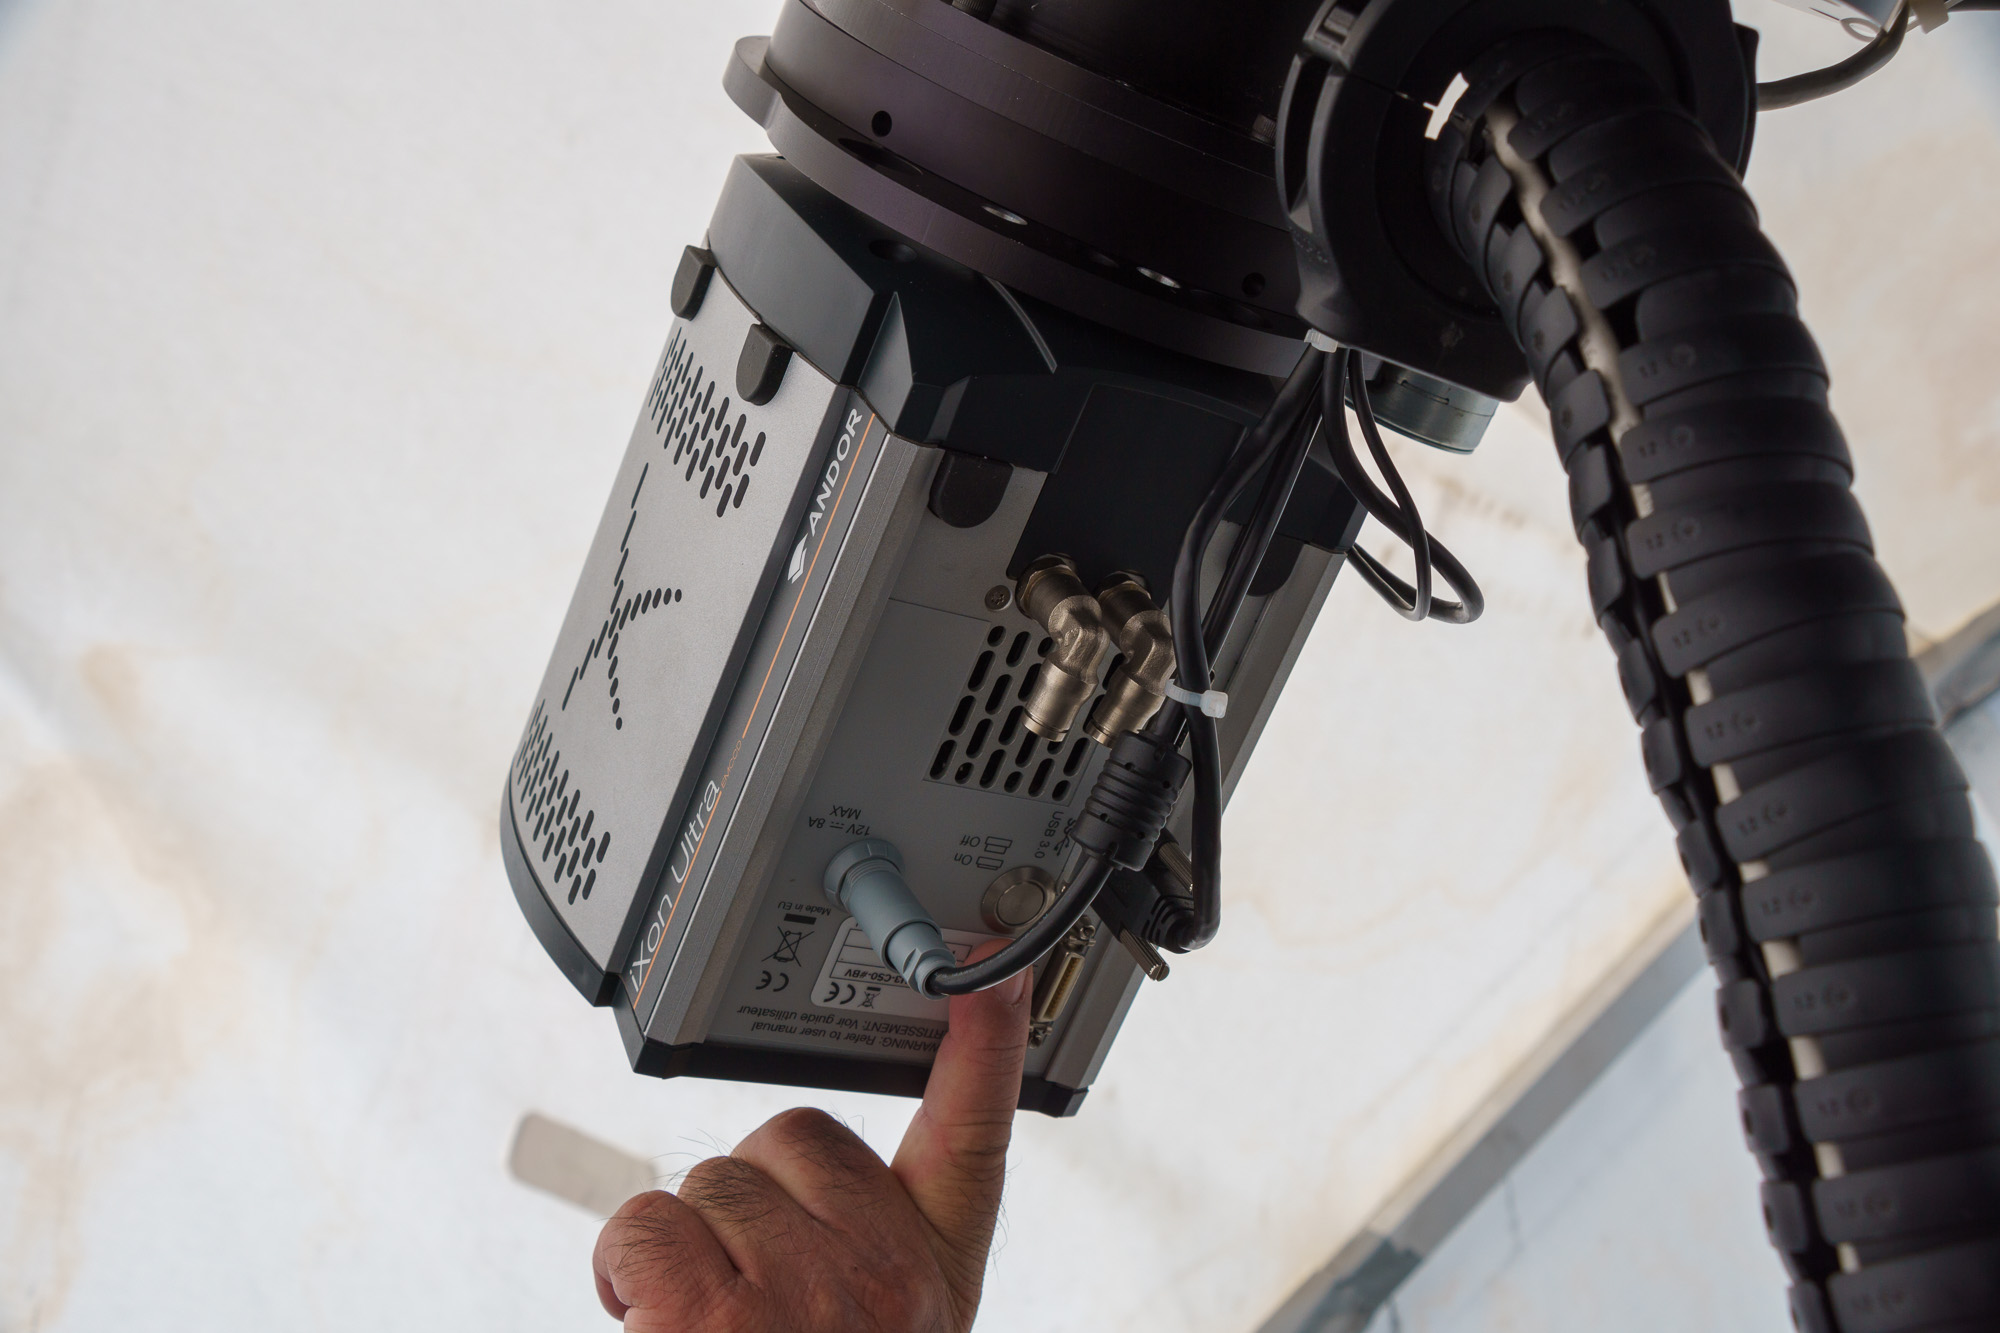
\includegraphics[width=0.8\linewidth]{figures/huitzi-detector-power-button.jpg}
\end{center}
\caption{The detector power button.}
\label{figure:huitzi-detector-power-button}
\end{figure*}

\begin{figure*}
\begin{center}
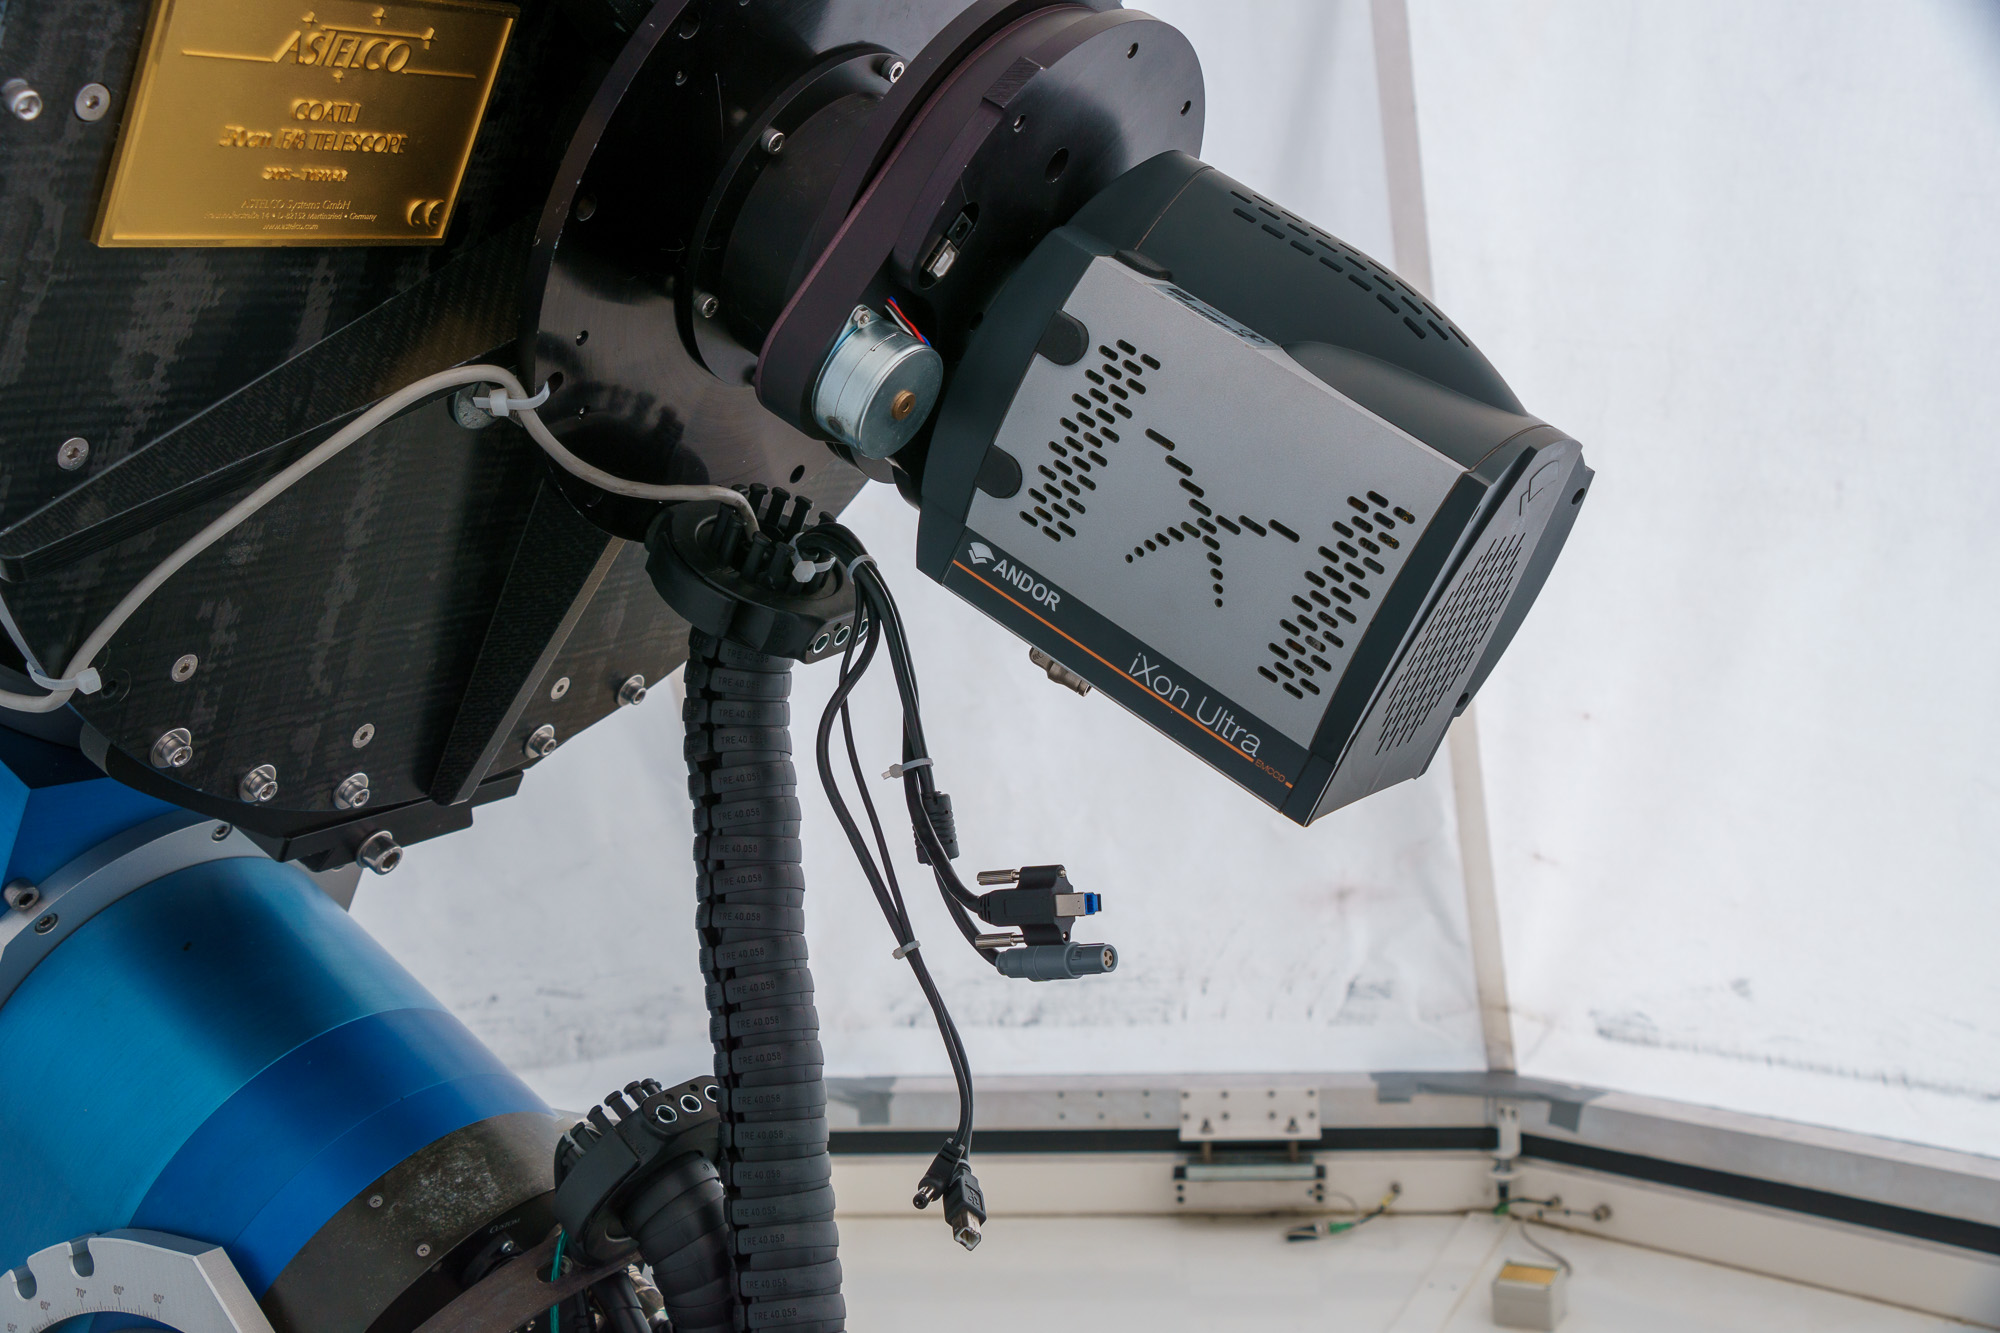
\includegraphics[width=0.8\linewidth]{figures/huitzi-cables-disconnected.jpg}
\end{center}
\caption{The disconnected detector and filter wheel USB and power cables.}
\label{figure:huitzi-cables-disconnected}
\end{figure*}

\begin{figure*}
\begin{center}
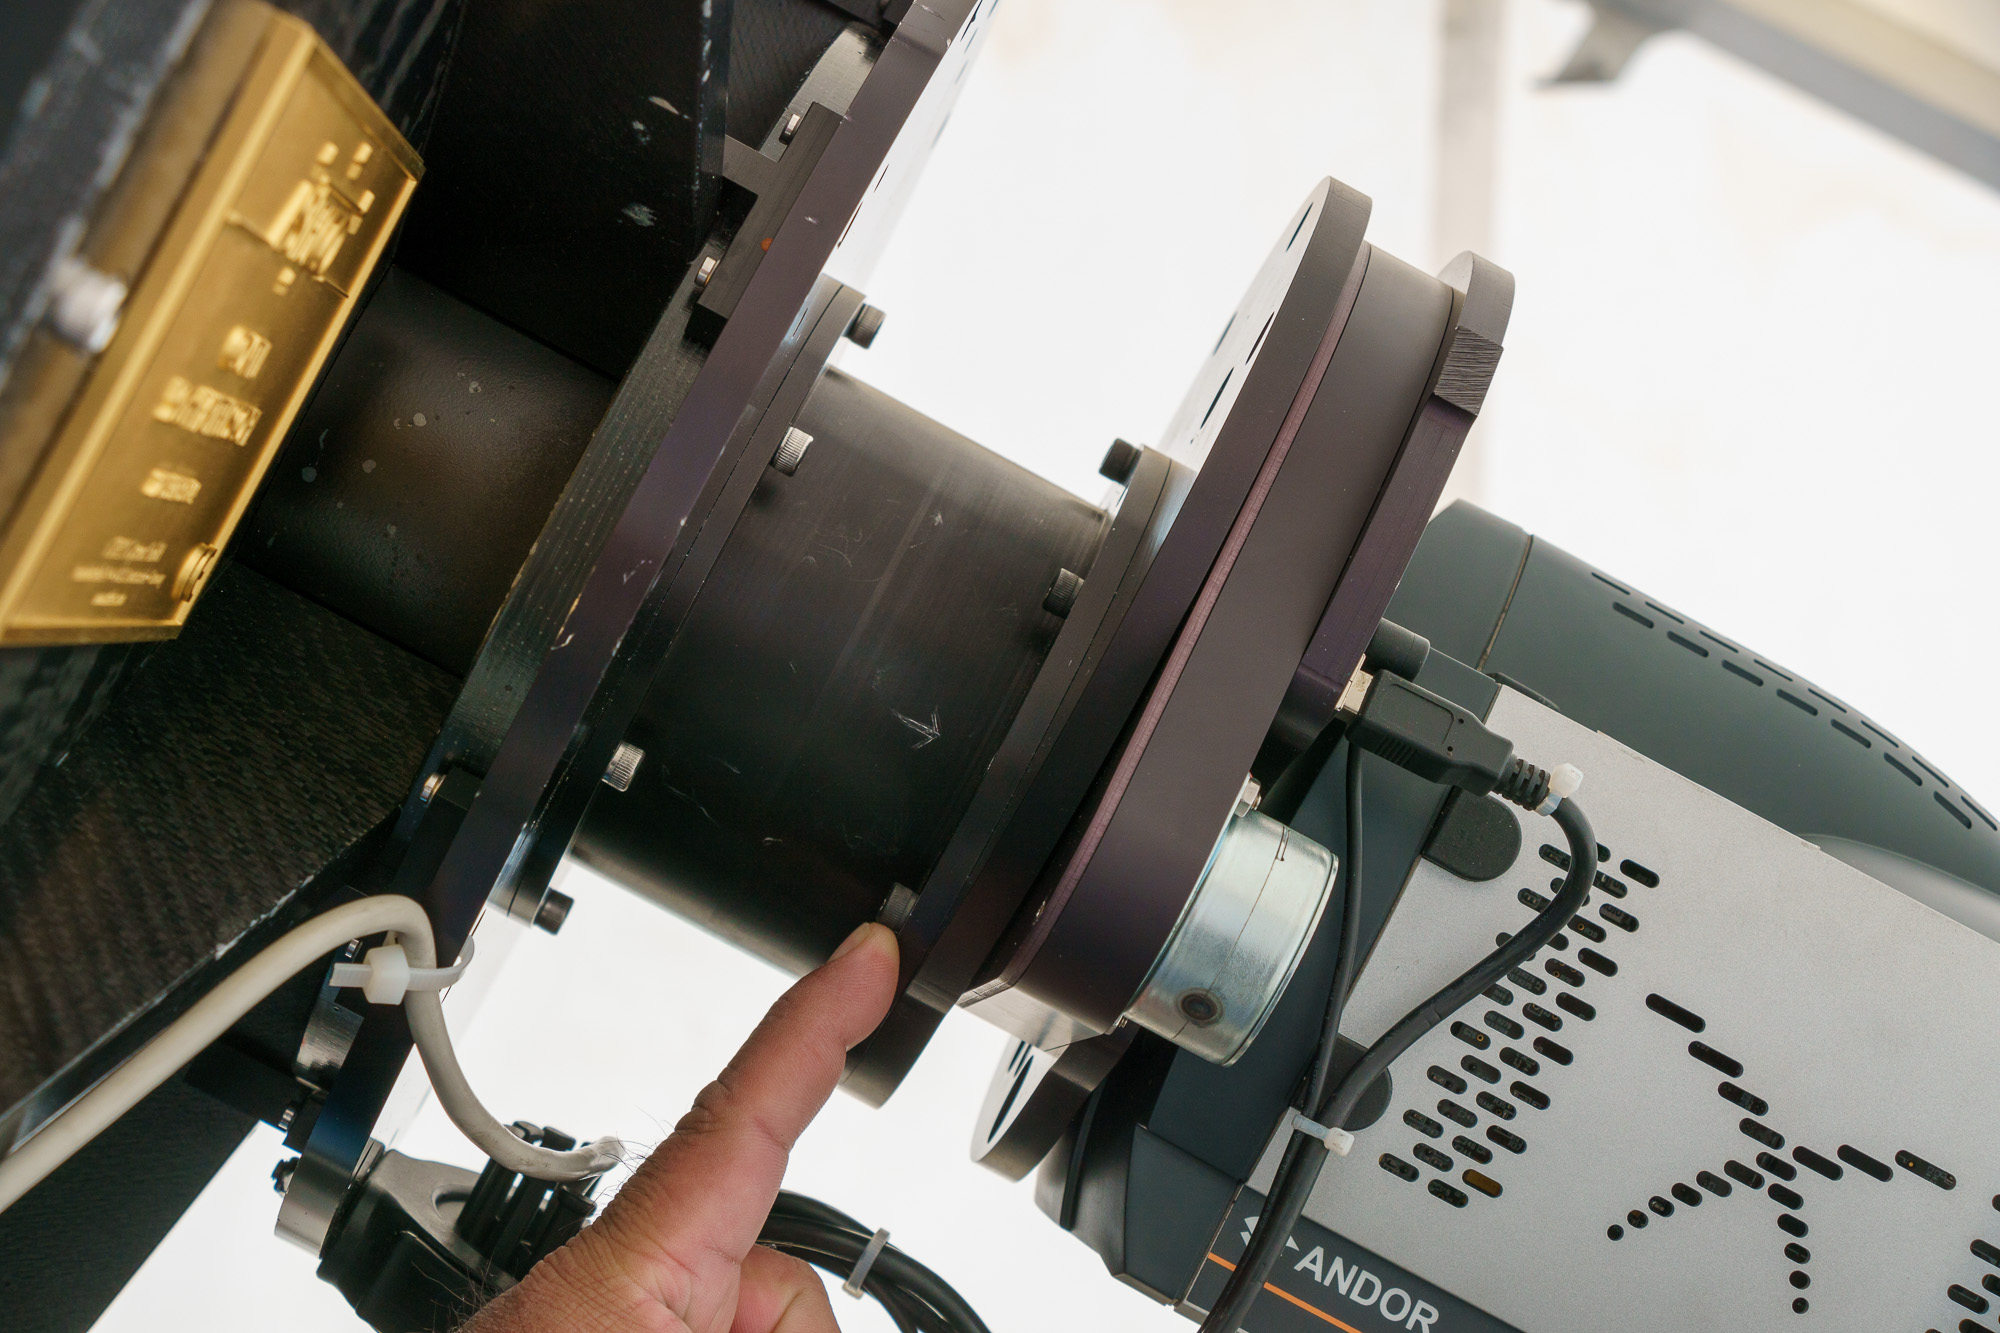
\includegraphics[width=0.8\linewidth]{figures/huitzi-mounting-screws.jpg}
\end{center}
\caption{The six screws that hold the filter wheel and detector to the separator barrel. Note the arrow scratched on the separator barrel that aligns with a similar barrel on the front filter wheel plate.}
\label{figure:huitzi-mounting-screws}
\end{figure*}

\begin{figure*}
\begin{center}
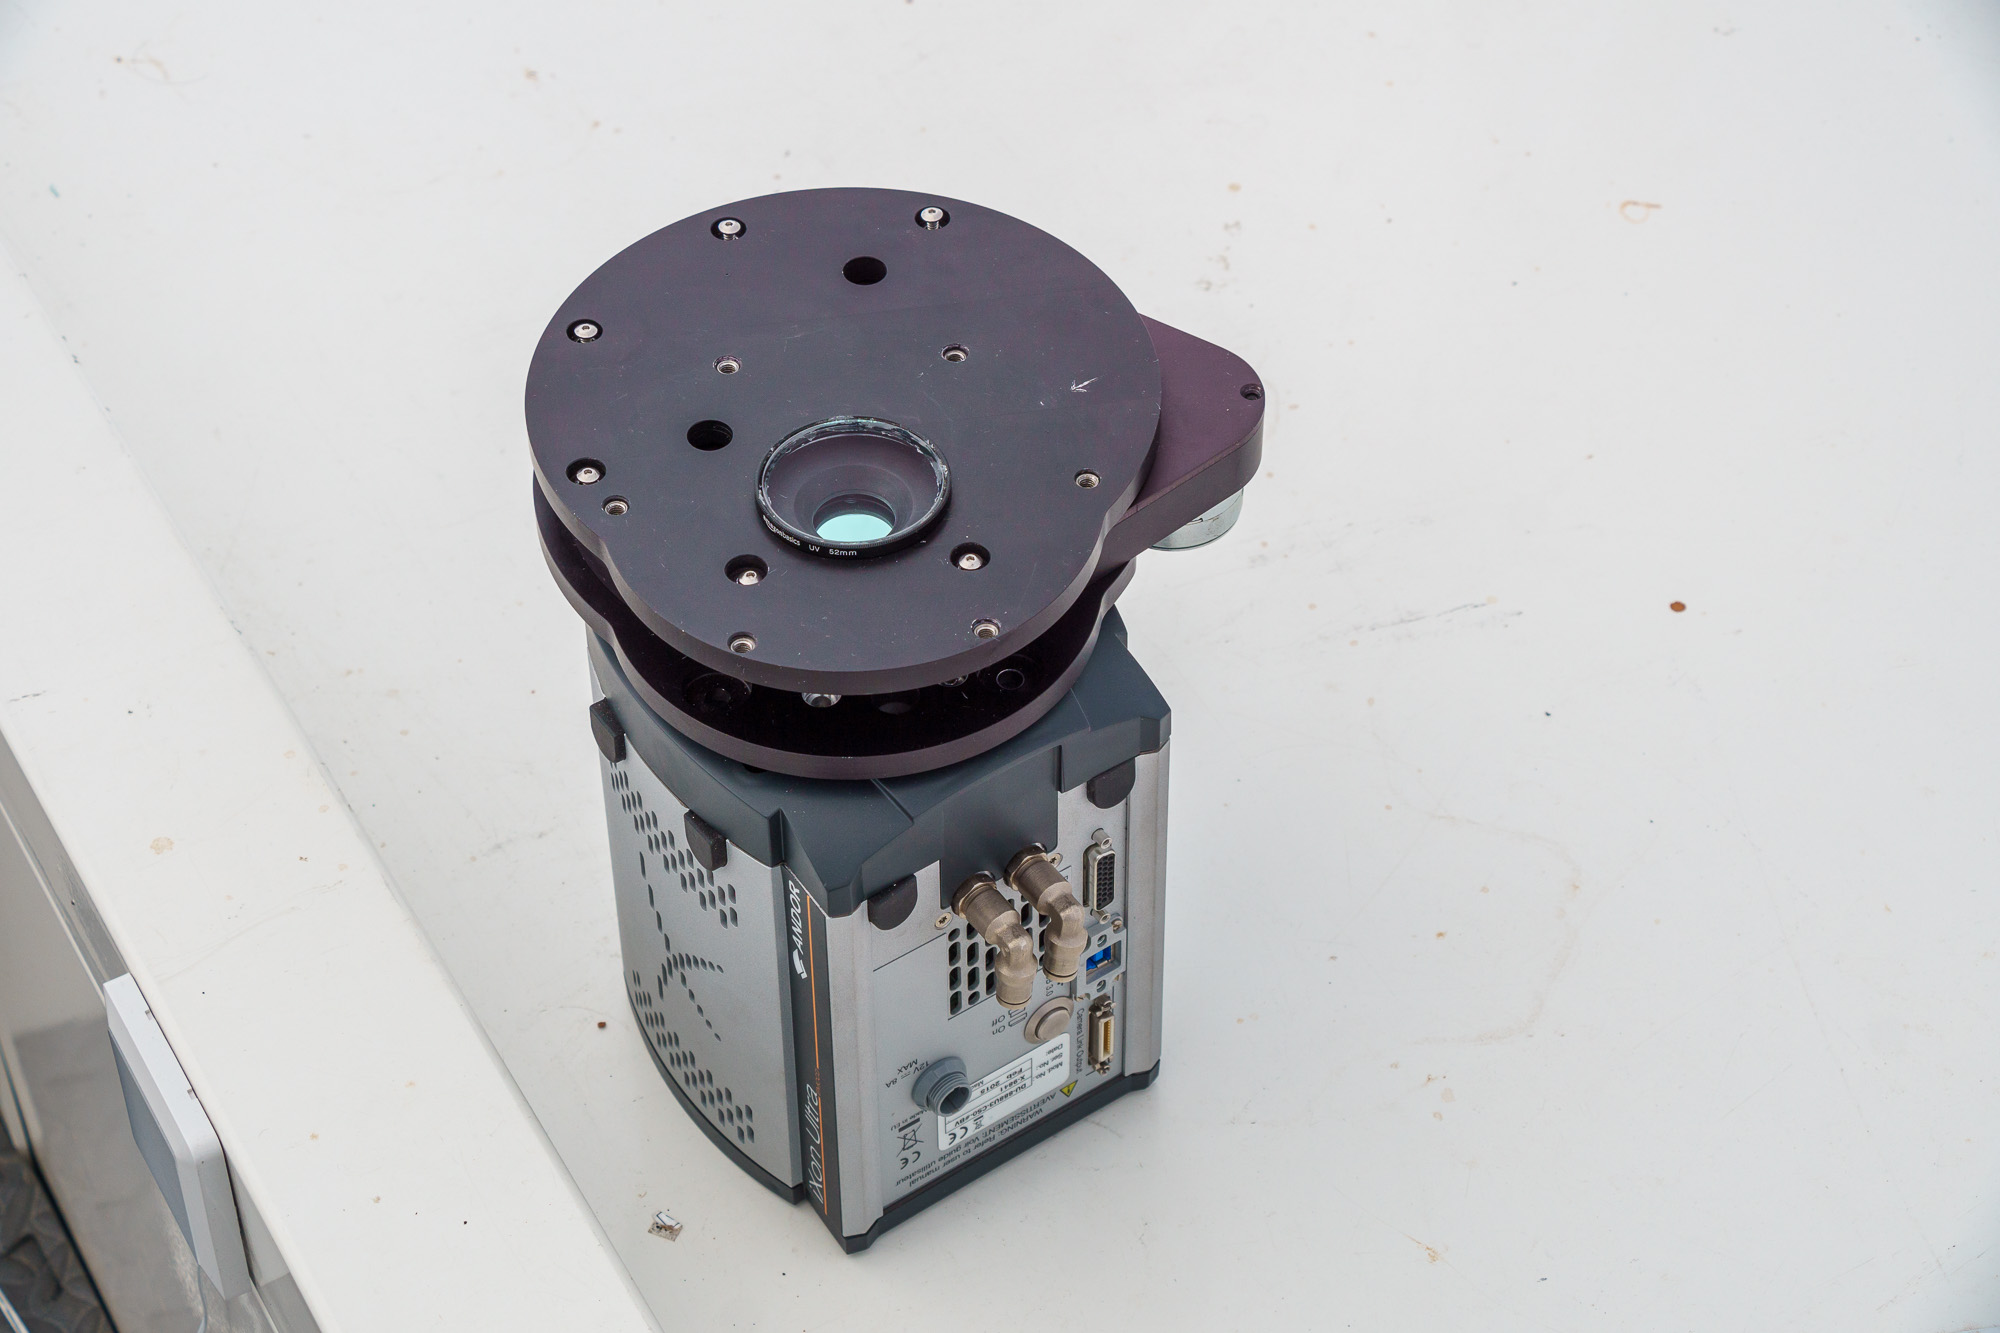
\includegraphics[width=0.8\linewidth]{figures/huitzi-off-telescope.jpg}
\end{center}
\caption{The dismounted detector and filter wheel resting on the rear surface of the detector. The six screws that hold the filter wheel between the front and rear plates can be seen here.}
\label{figure:huitzi-off-telescope}
\end{figure*}

\begin{figure*}
\begin{center}
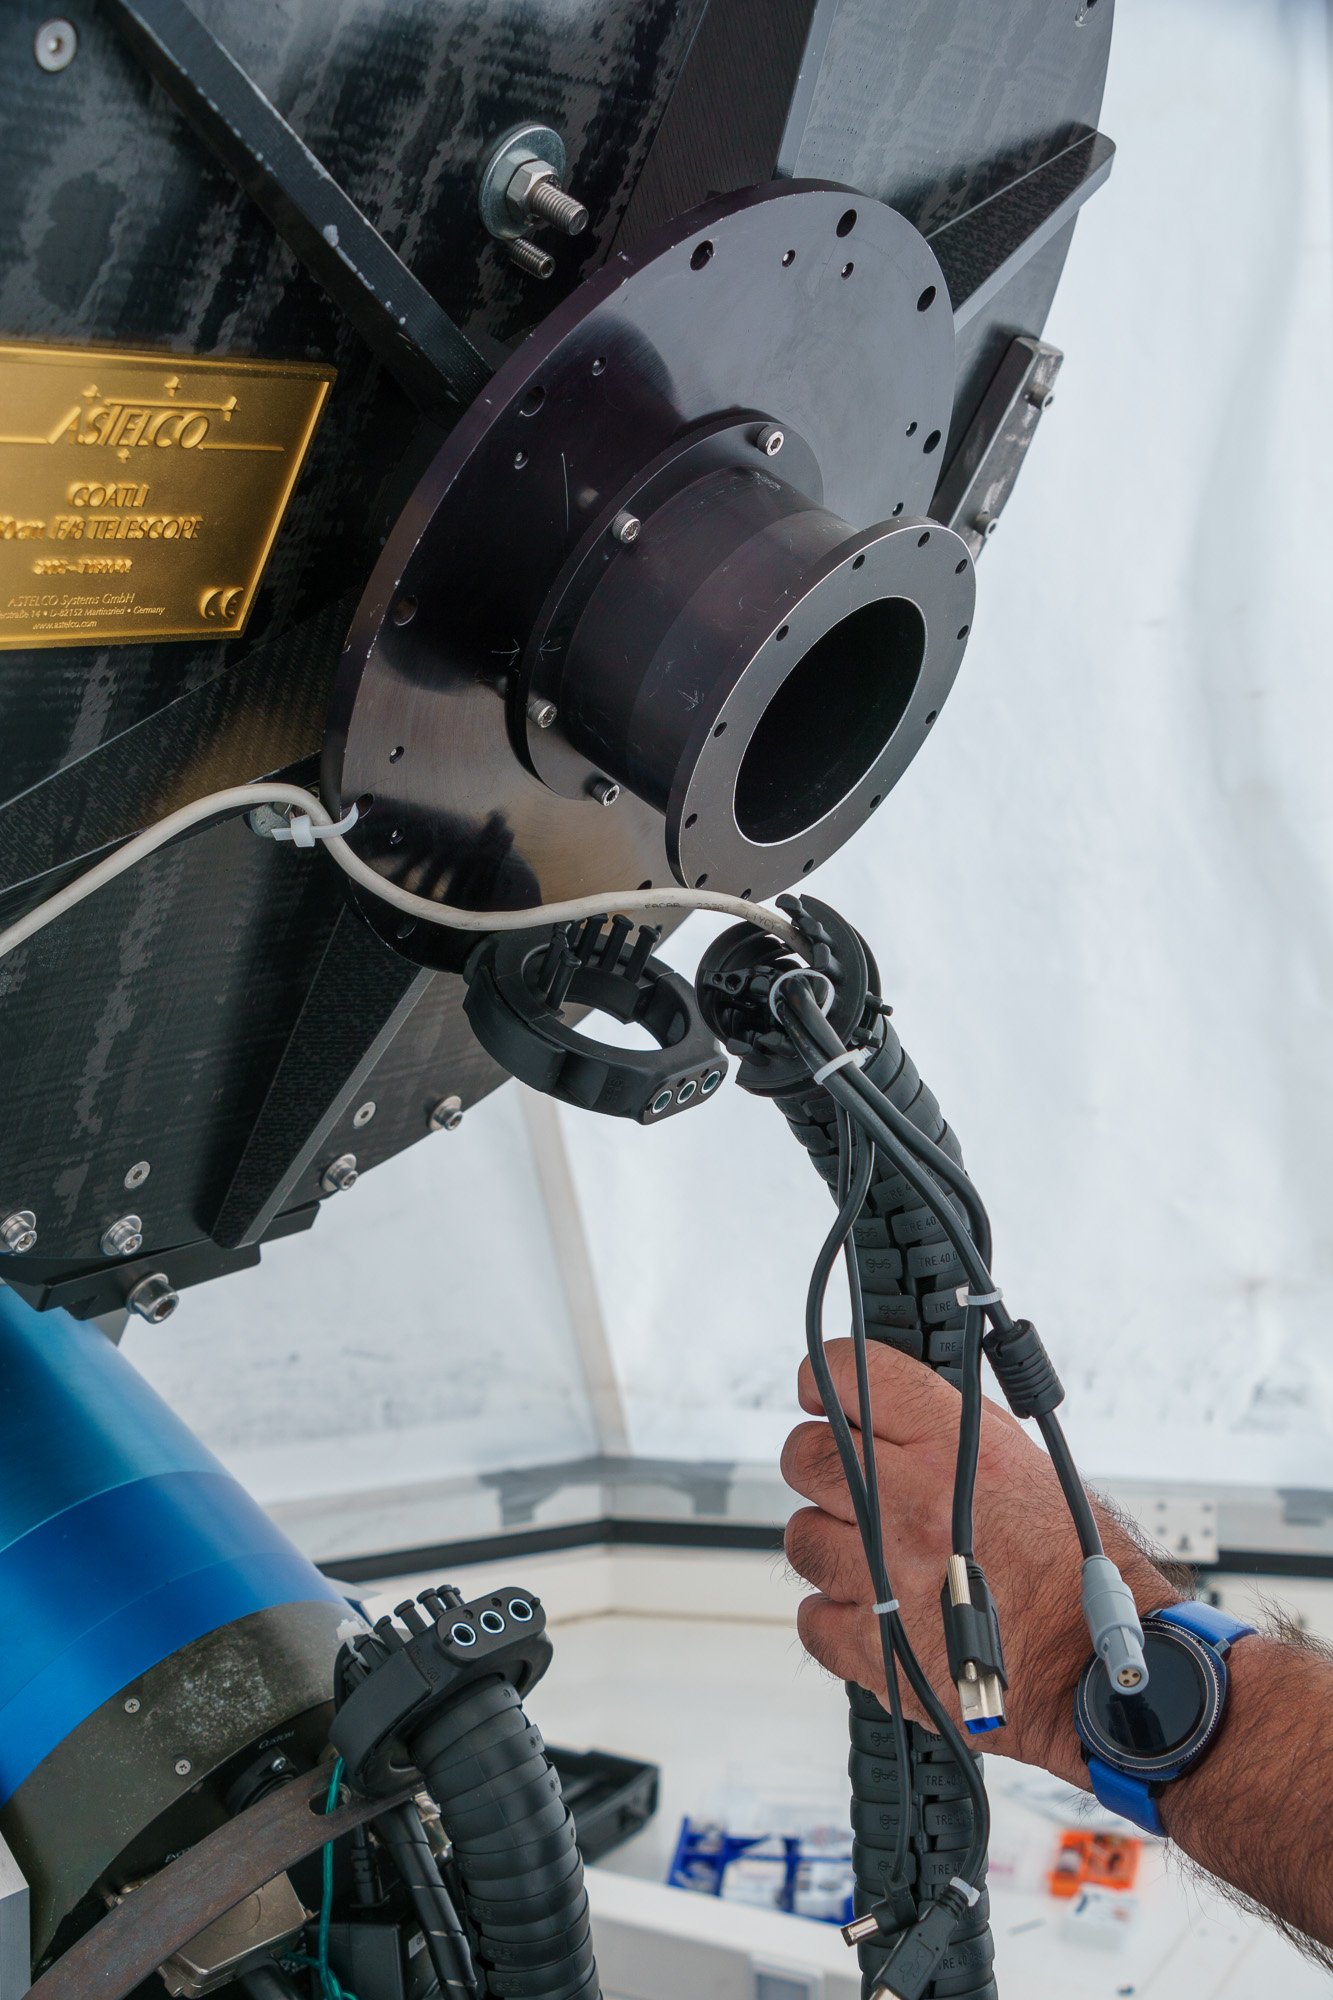
\includegraphics[width=0.3\linewidth]{figures/huitzi-operating-off-telescope-a.jpg}
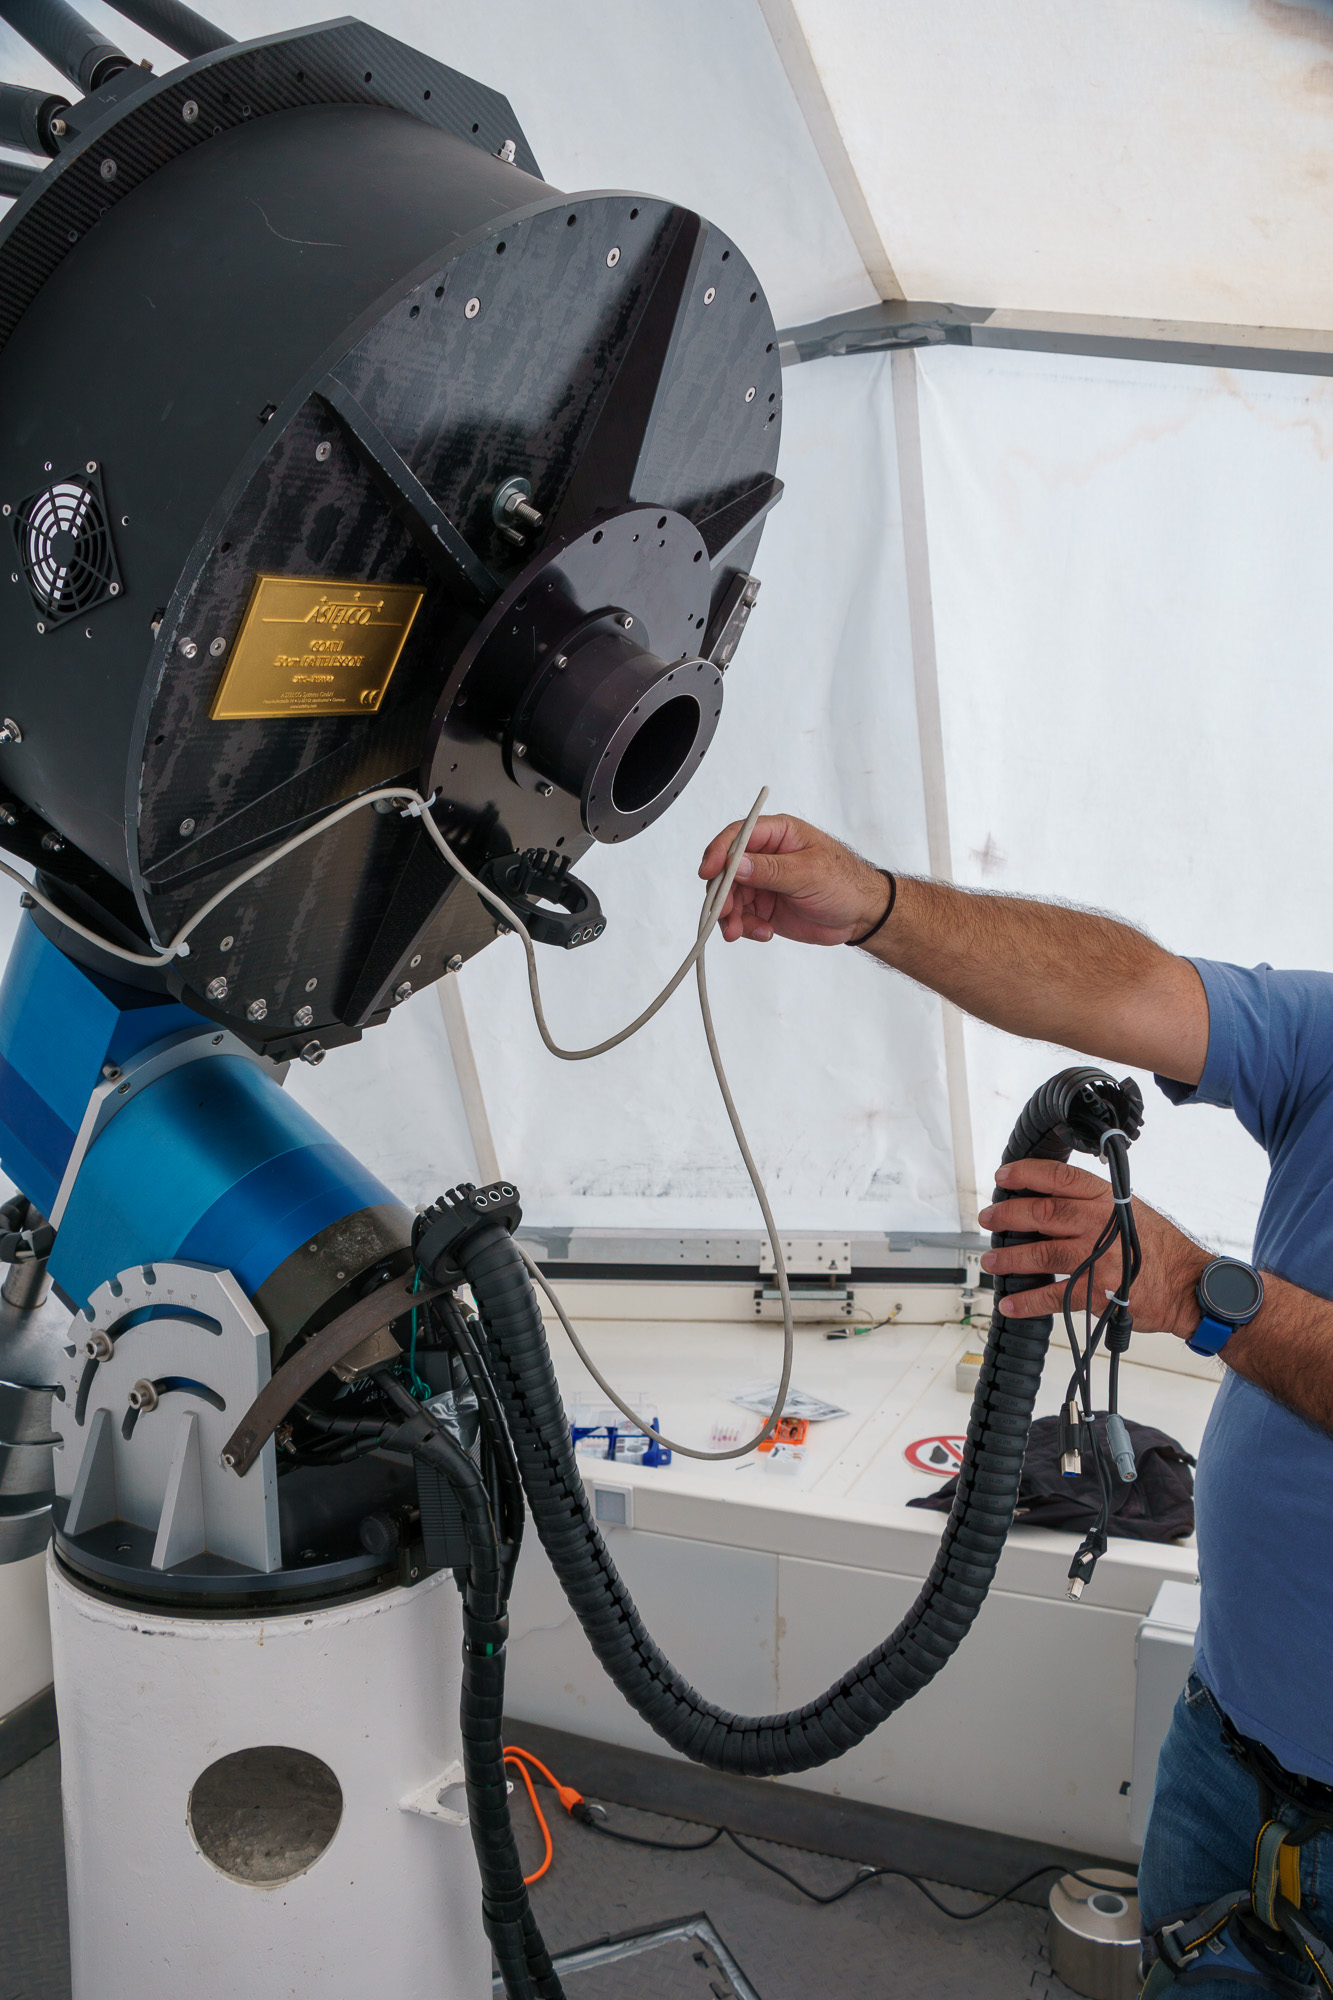
\includegraphics[width=0.3\linewidth]{figures/huitzi-operating-off-telescope-b.jpg}
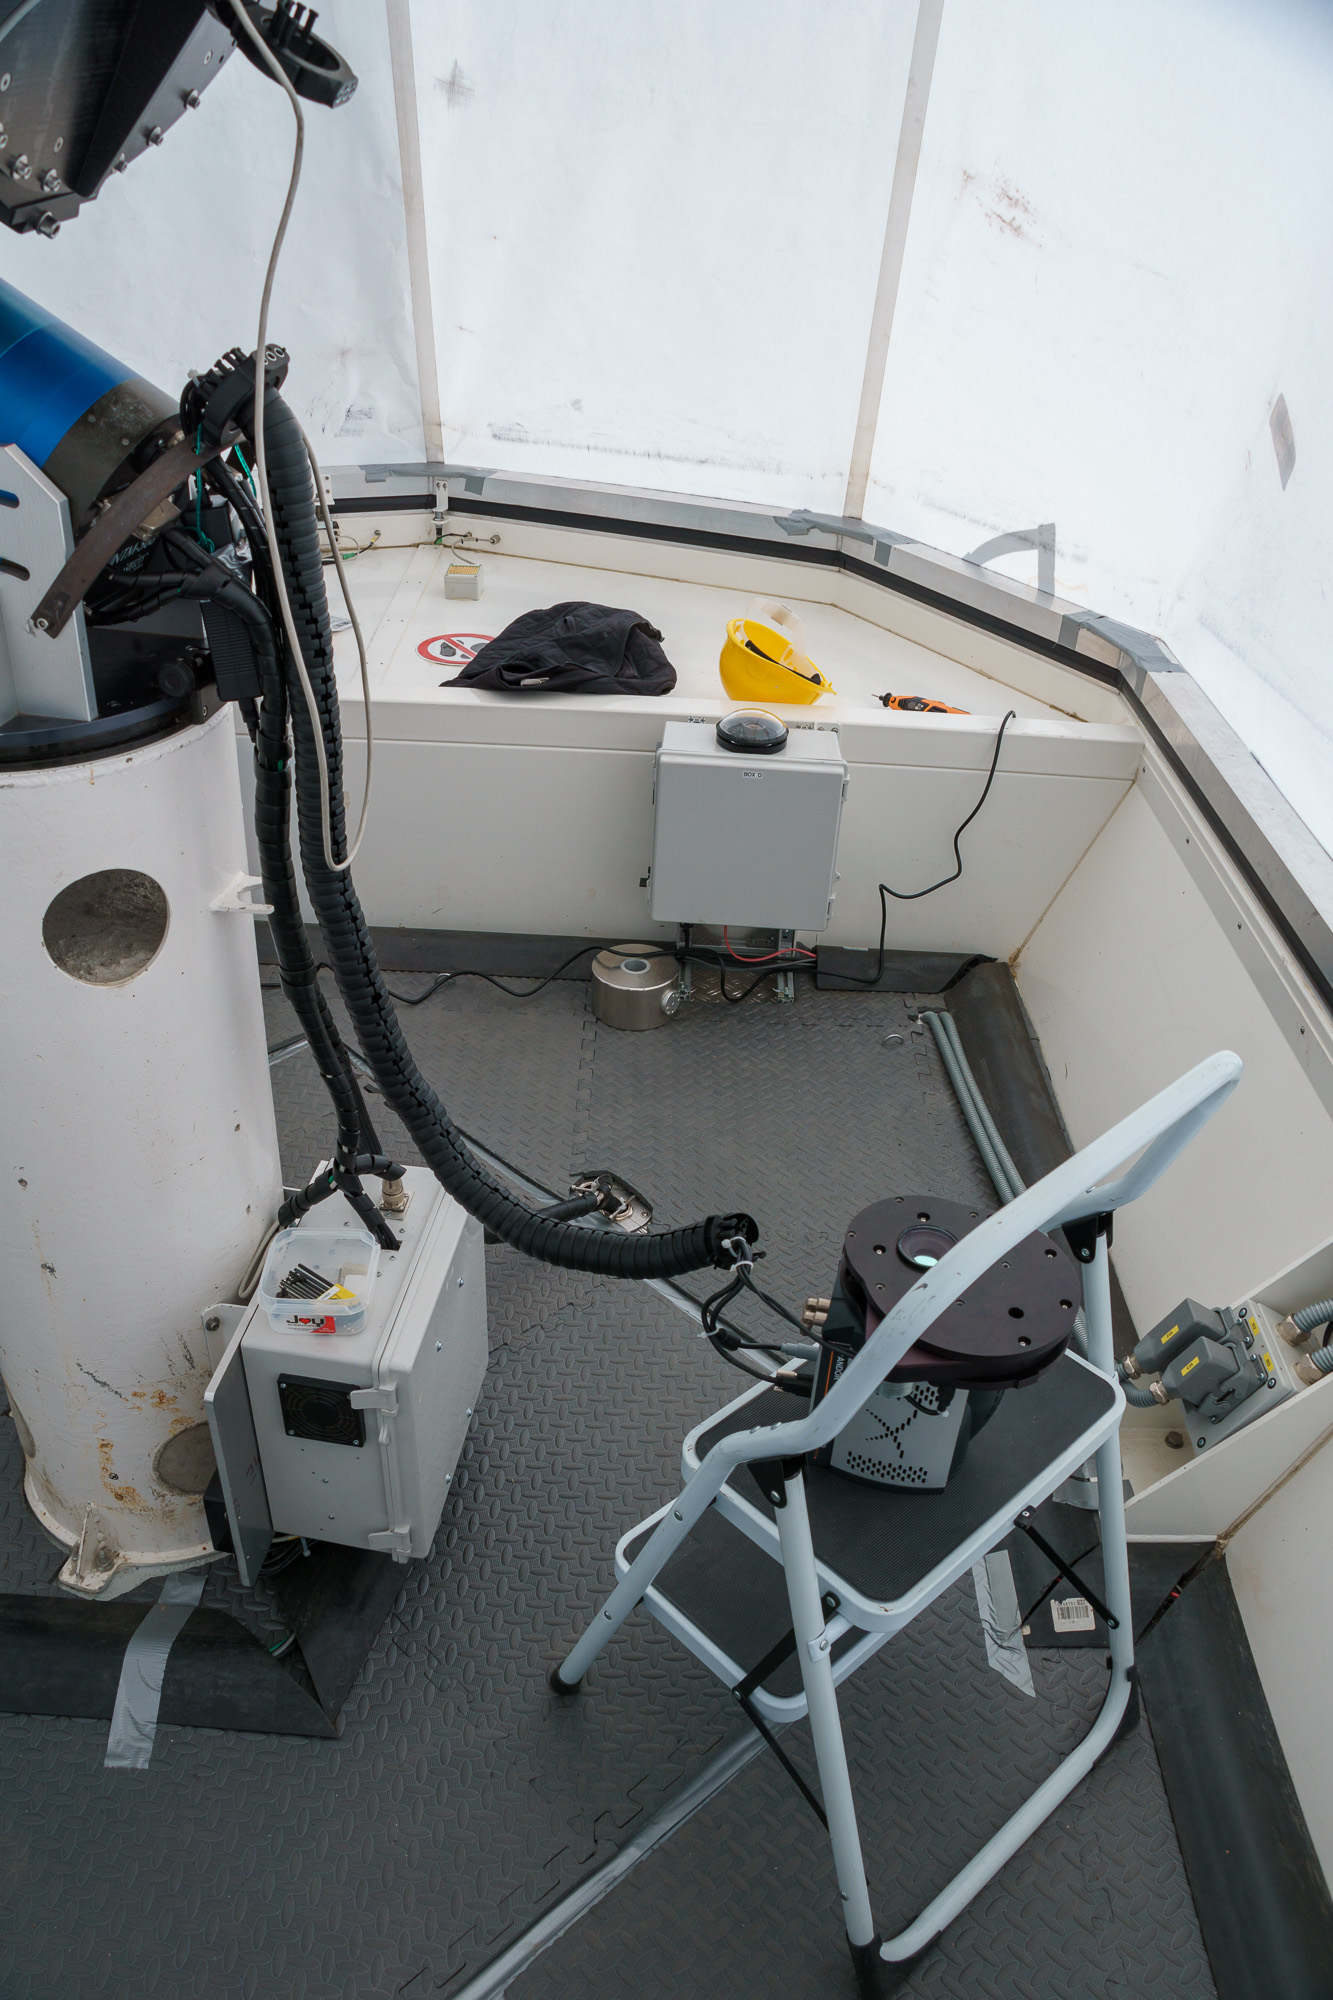
\includegraphics[width=0.3\linewidth]{figures/huitzi-operating-off-telescope-c.jpg}
\end{center}
\caption{Operating the instrument off the telescope. Disconnect the Igus Triflex chain, remove the white secondary cable, connect the instrument, and press the power button on the detector..}
\label{figure:huitzi-operating-off-telescope}
\end{figure*}

\begin{figure*}
\begin{center}
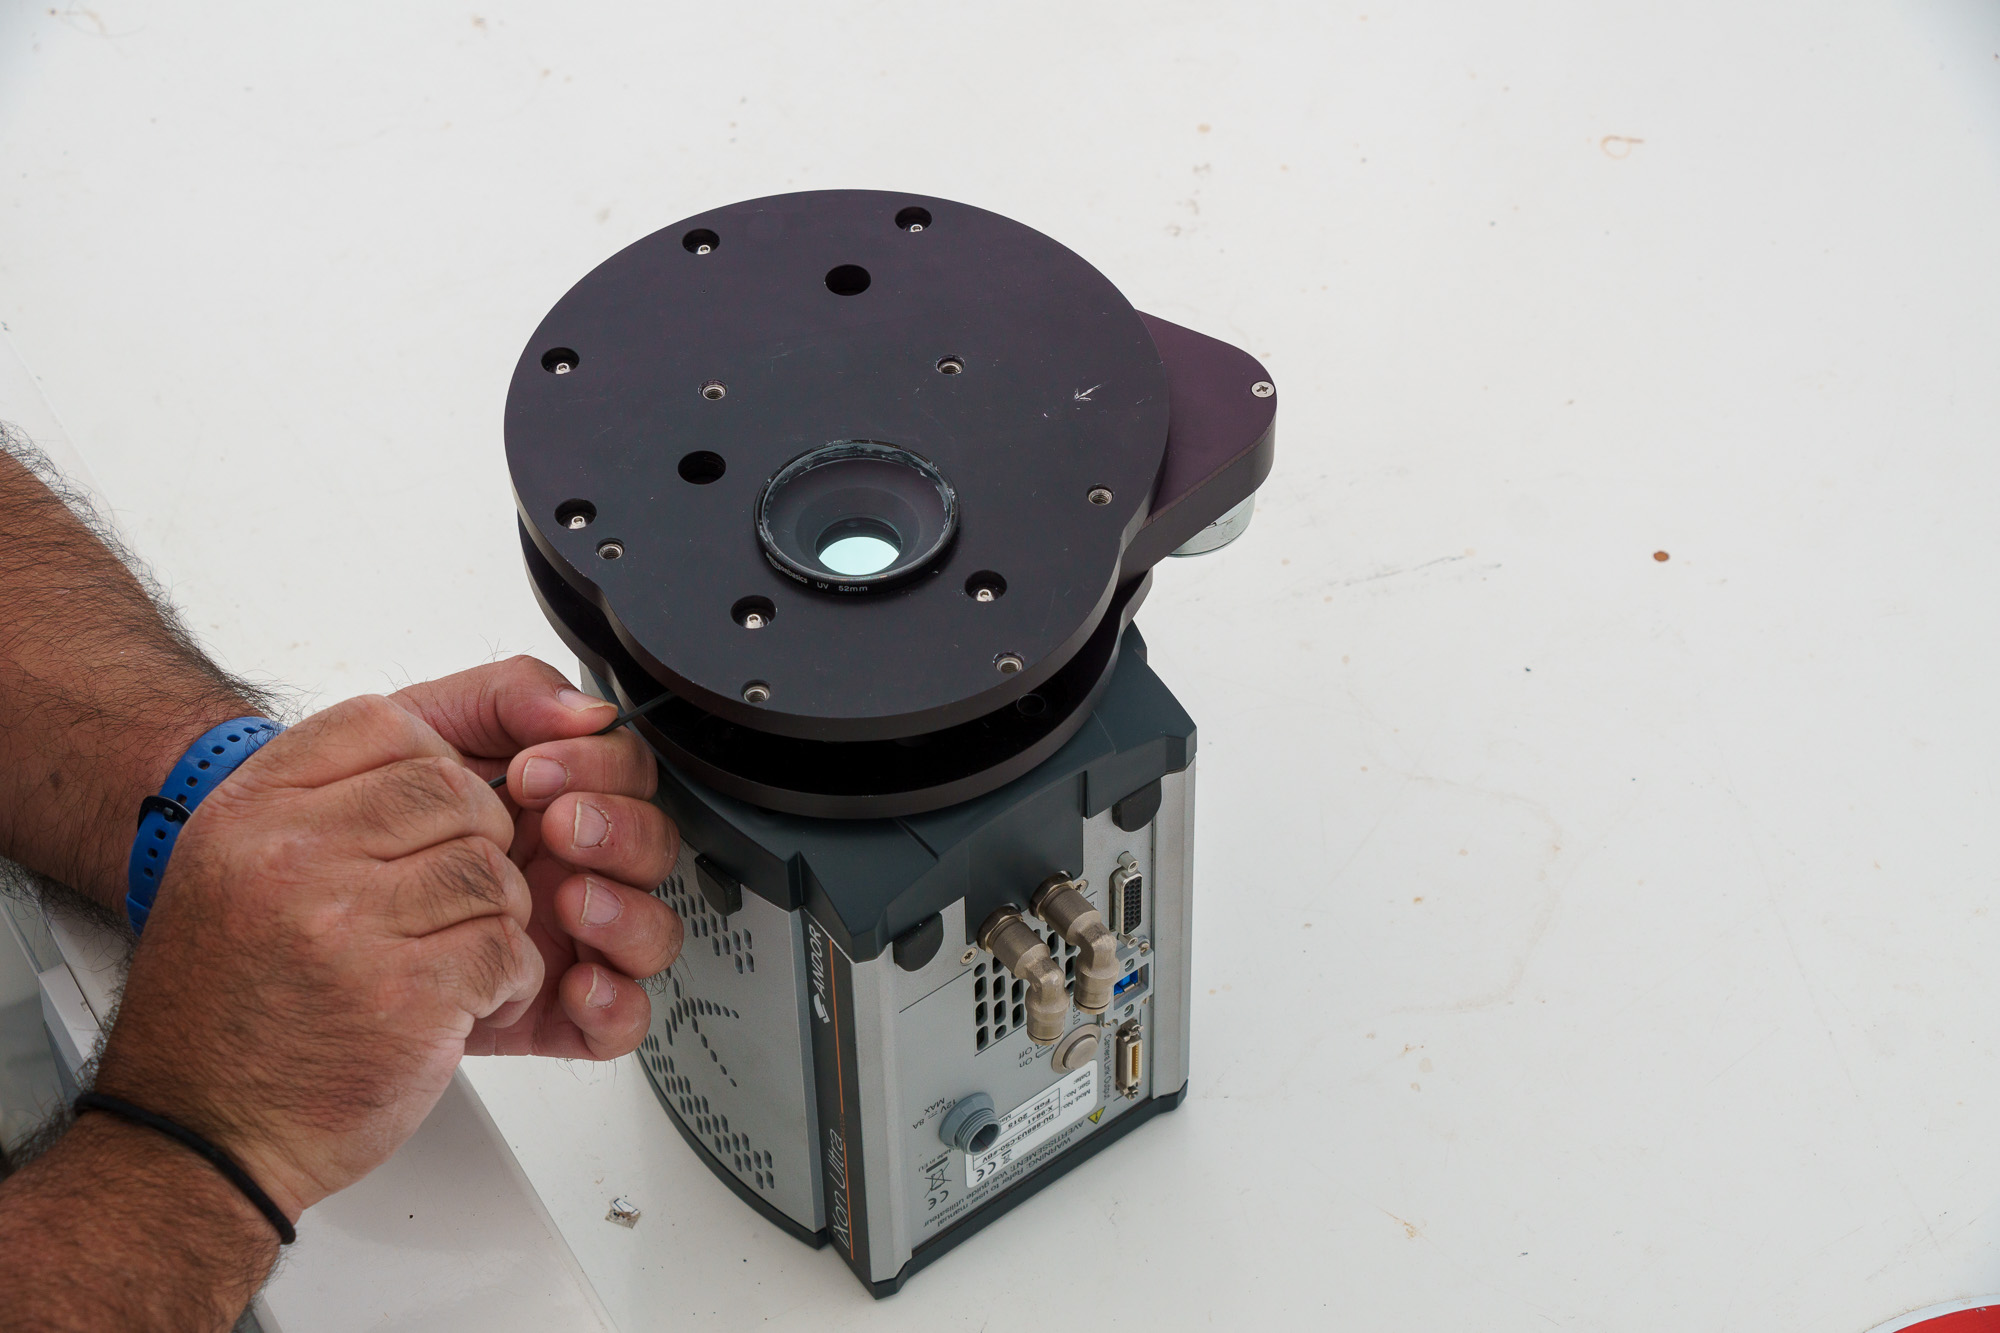
\includegraphics[width=0.8\linewidth]{figures/huitzi-set-screws-a.jpg}
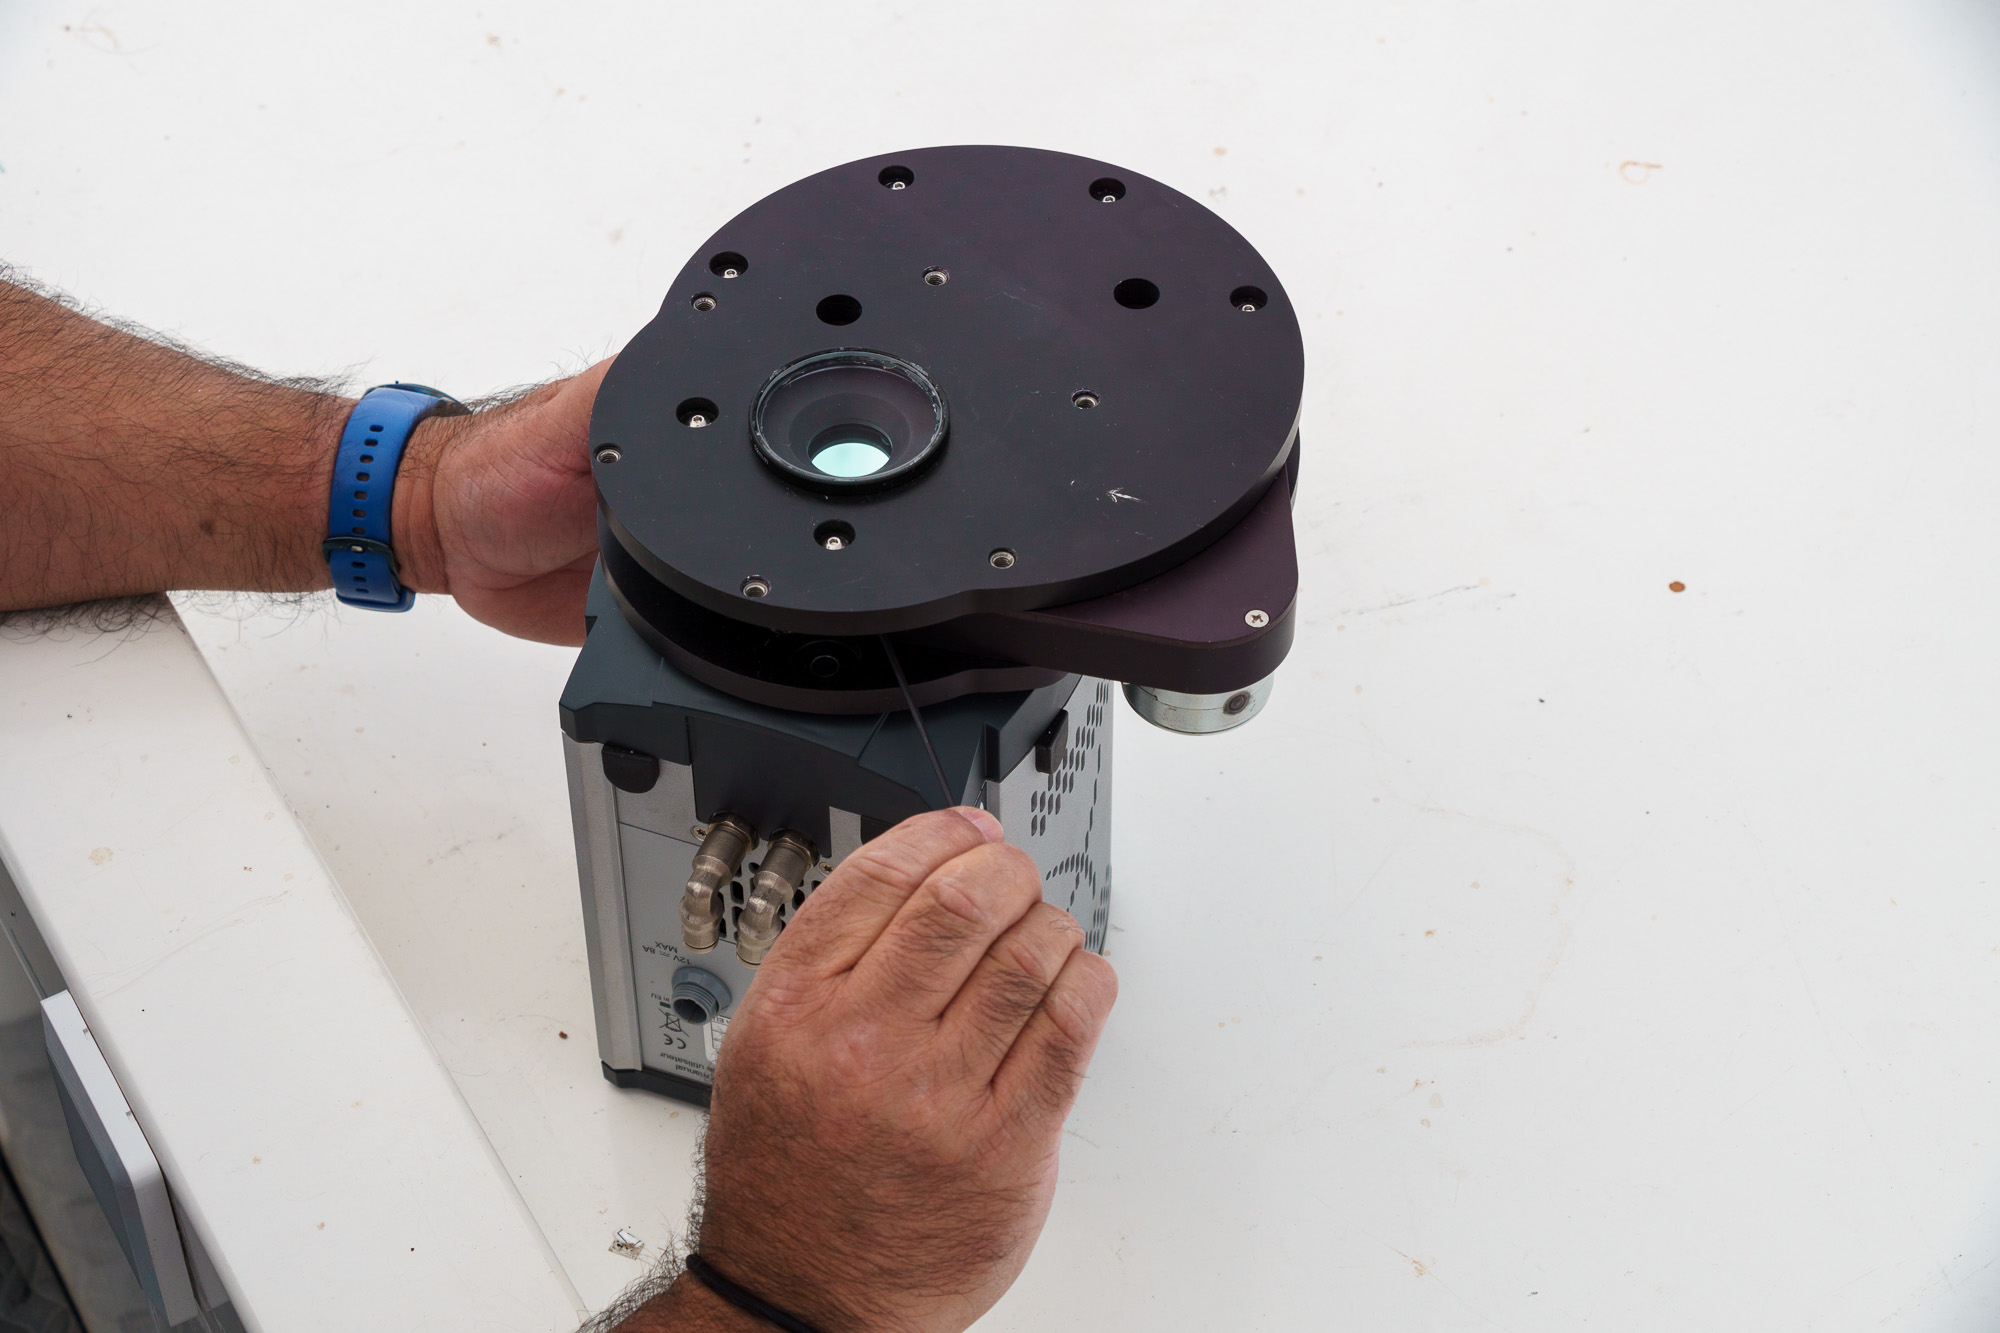
\includegraphics[width=0.8\linewidth]{figures/huitzi-set-screws-b.jpg}
\end{center}
\caption{The two set screws in the filter wheel.}
\label{figure:huitzi-set-screws}
\end{figure*}


\begin{figure*}
\begin{center}
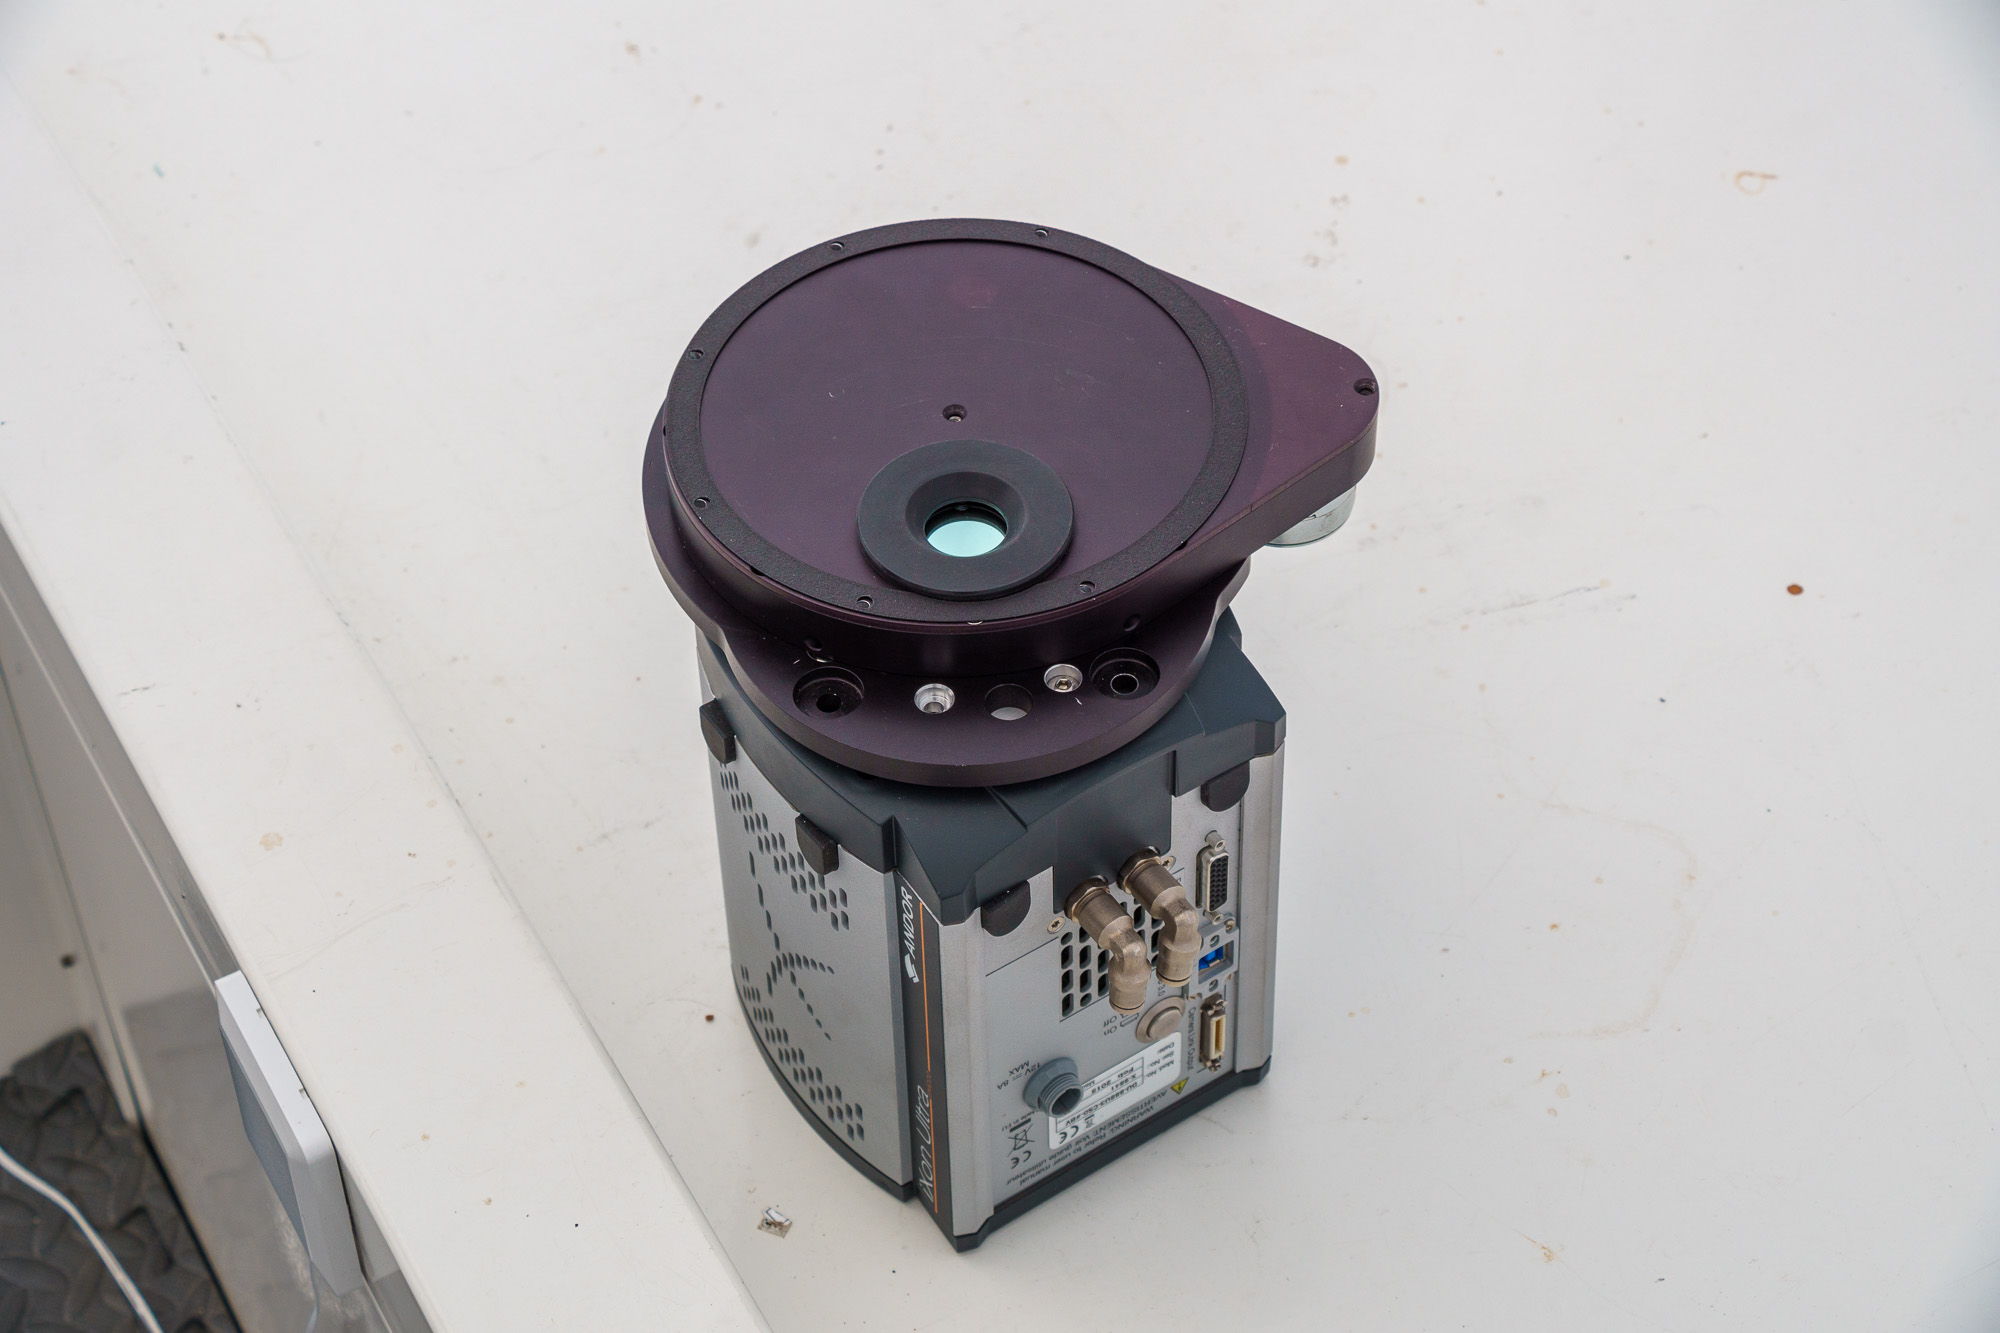
\includegraphics[width=0.8\linewidth]{figures/huitzi-without-front-plate.jpg}
\end{center}
\caption{The detector and filter wheel without the front plate.}
\label{figure:huitzi-without-front-plate}
\end{figure*}

\begin{figure*}
\begin{center}
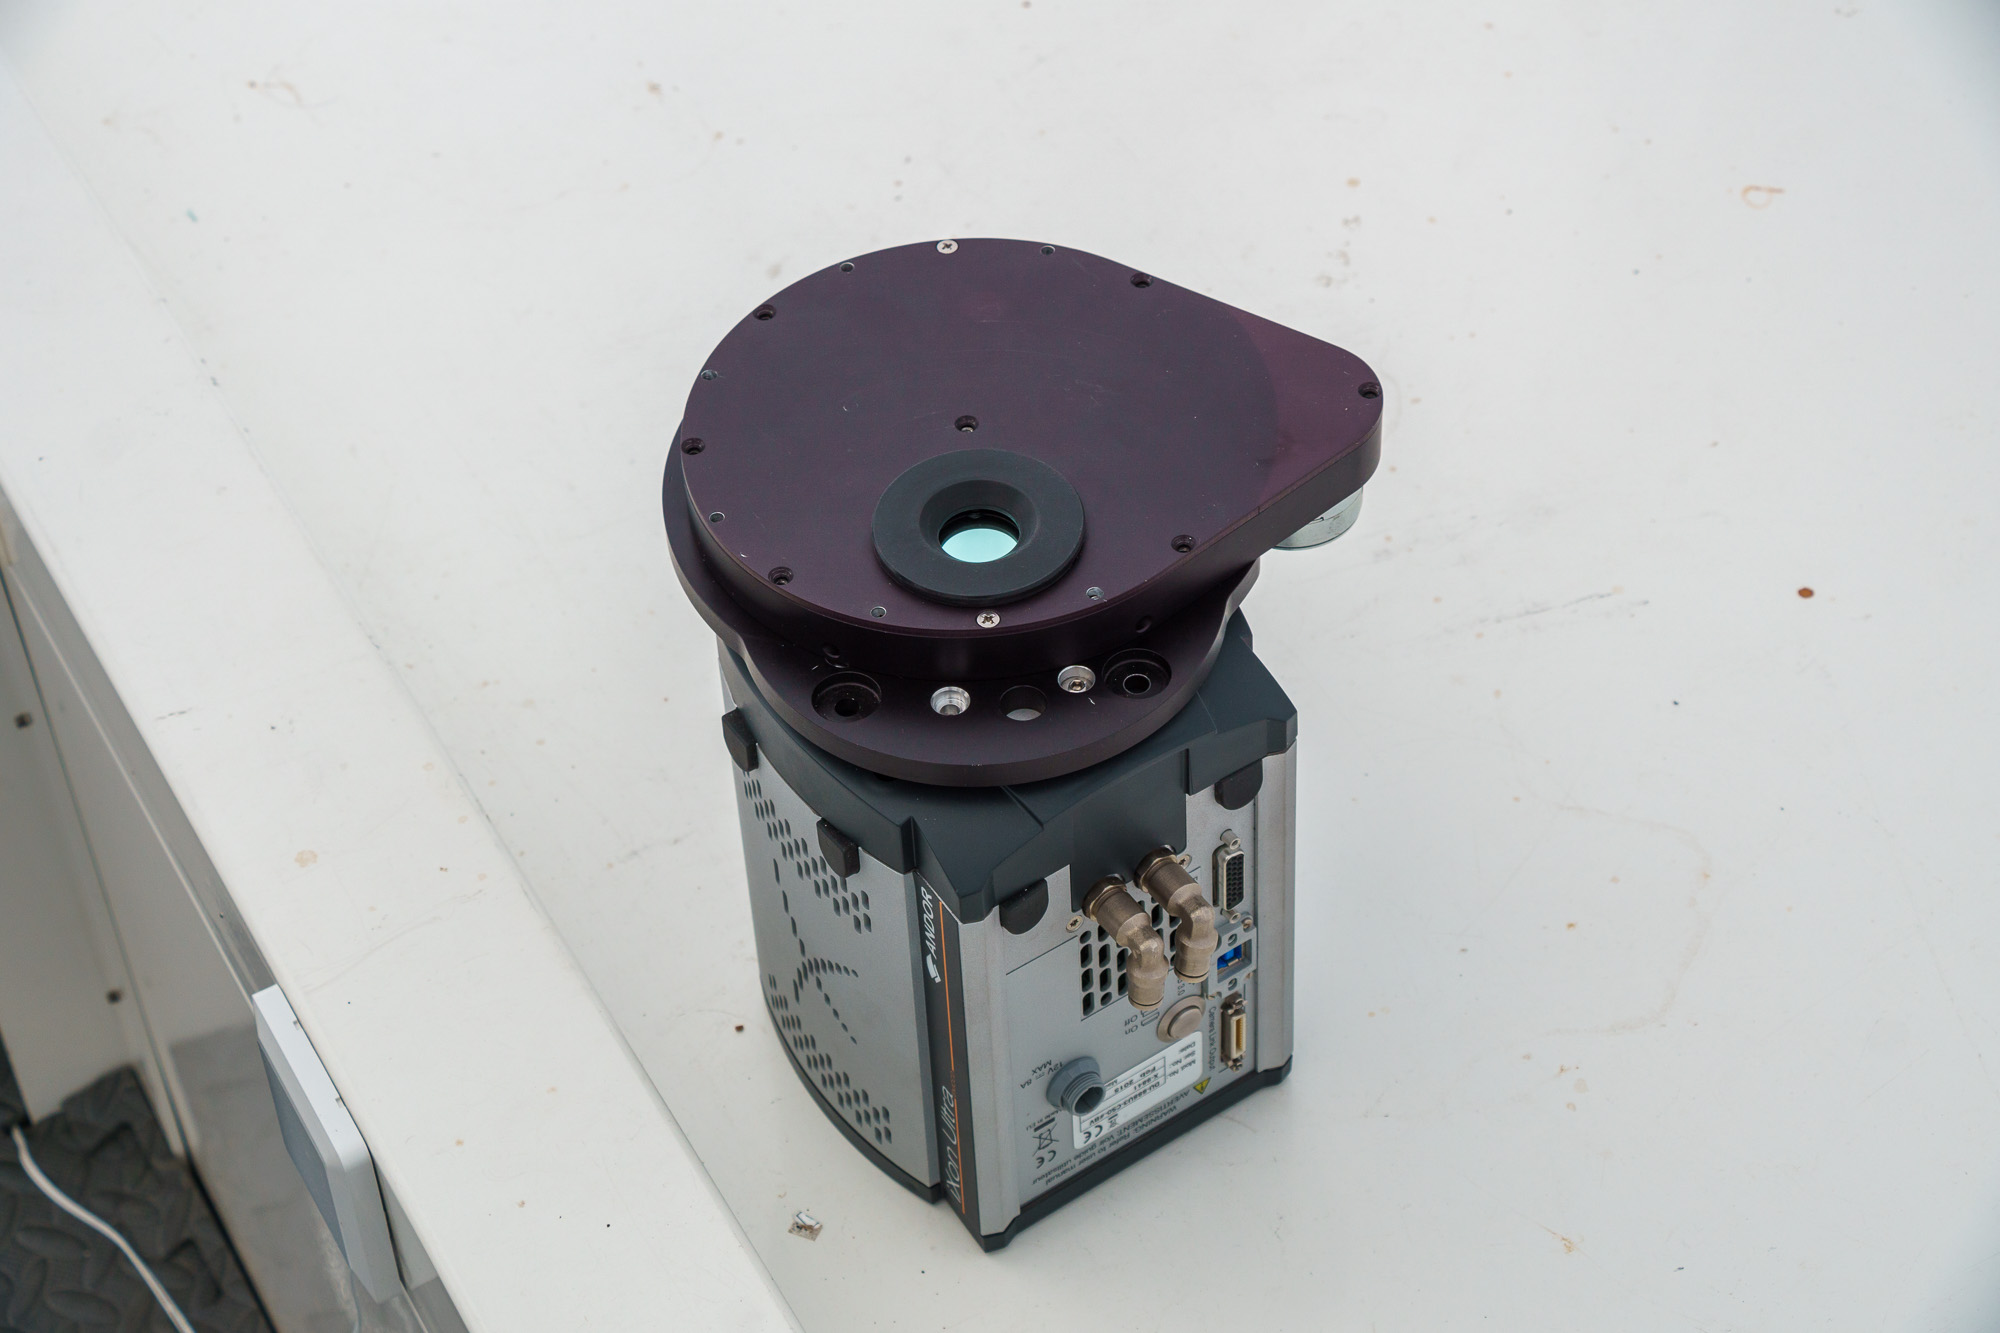
\includegraphics[width=0.8\linewidth]{figures/huitzi-without-spacer.jpg}
\end{center}
\caption{The detector and filter wheel without the spacer.}
\label{figure:huitzi-without-spacer}
\end{figure*}

\begin{figure*}
\begin{center}
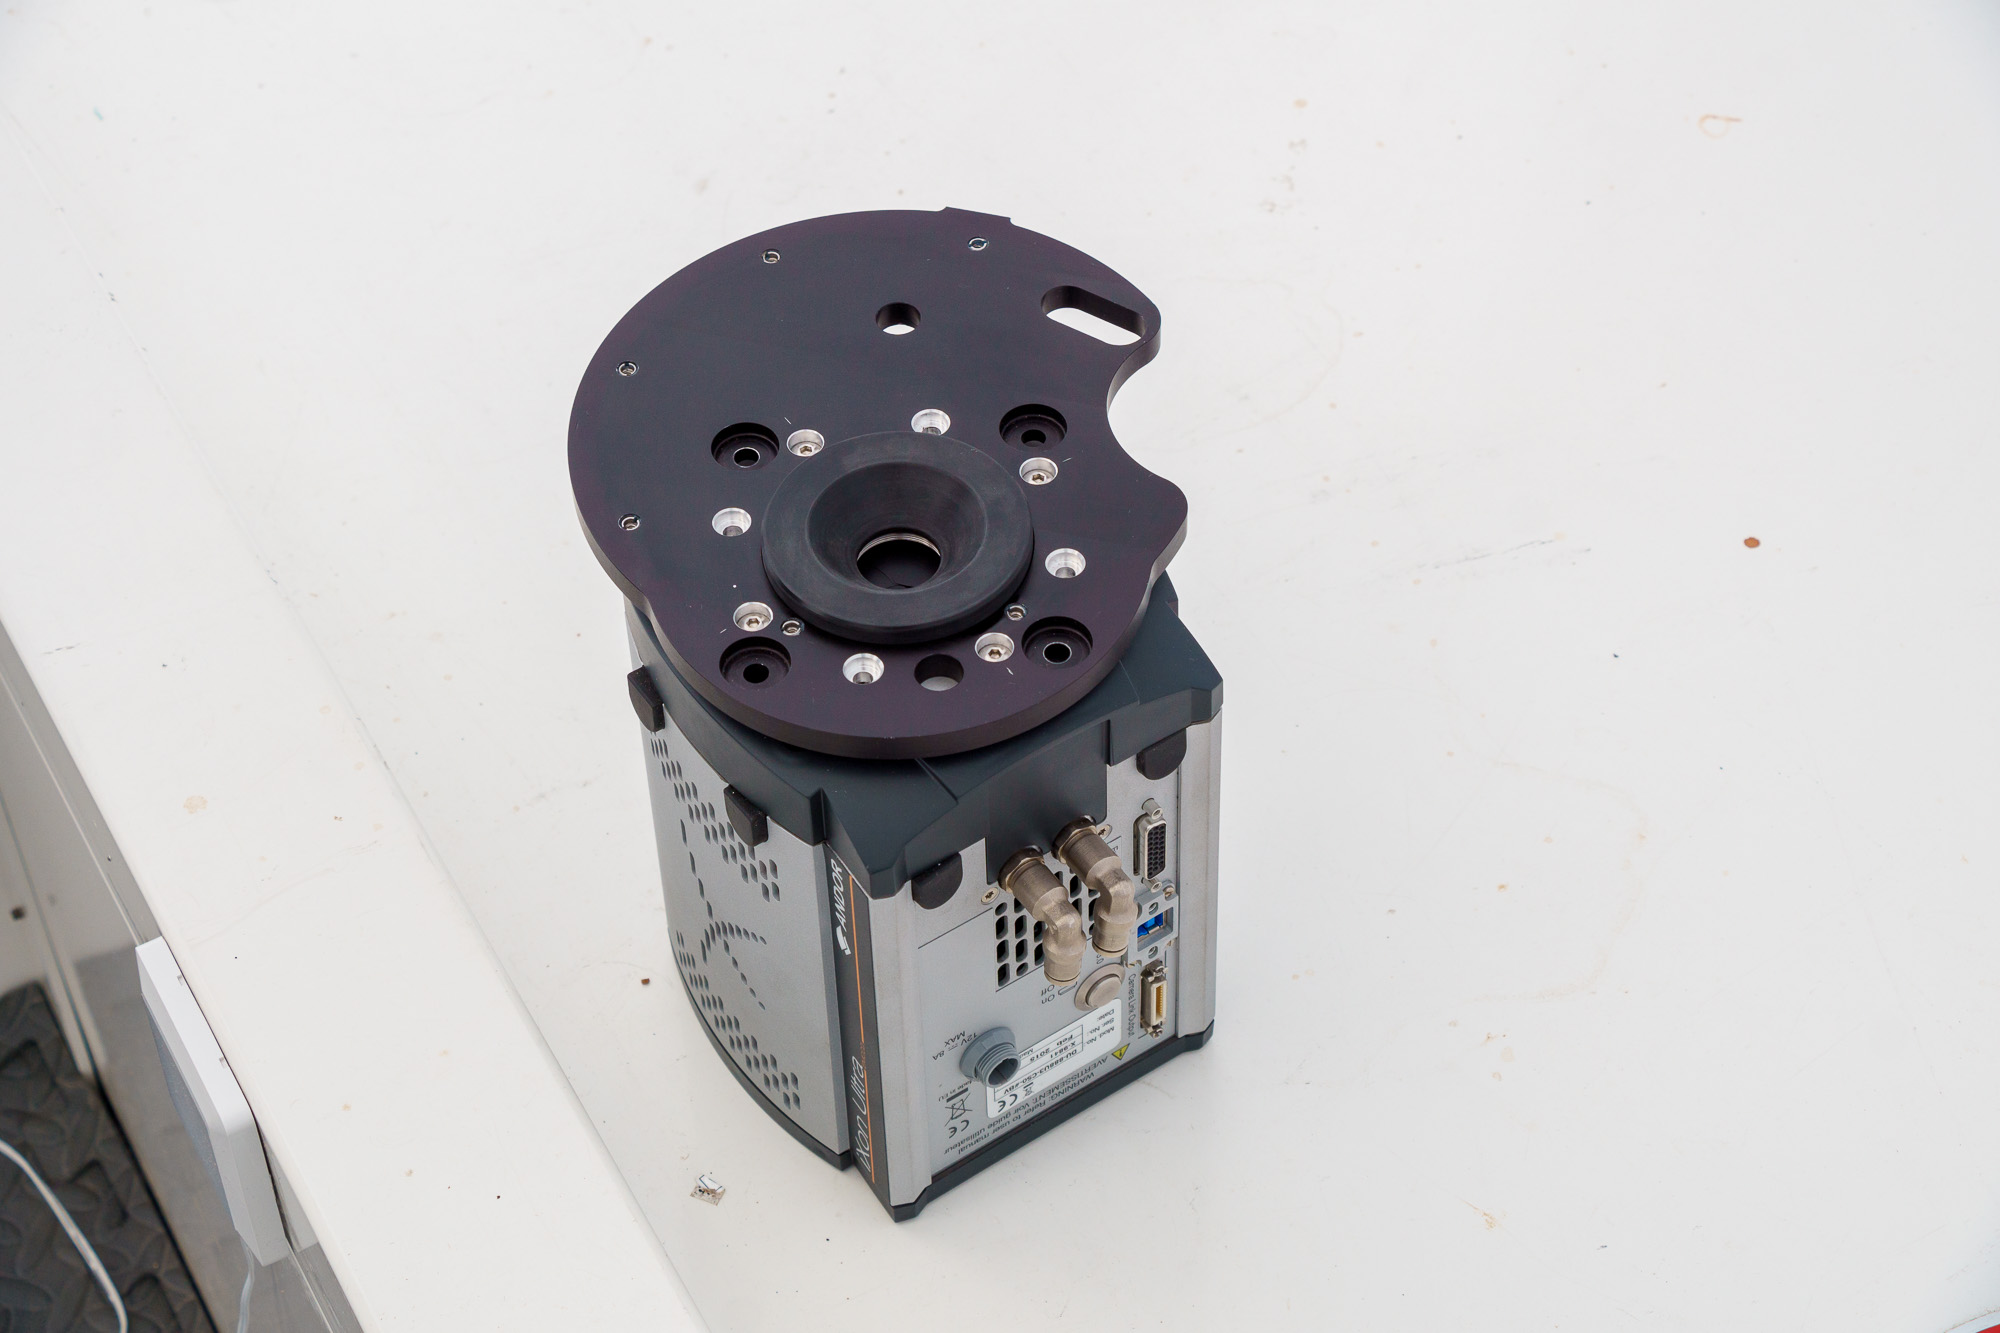
\includegraphics[width=0.8\linewidth]{figures/huitzi-without-filter-wheel.jpg}
\end{center}
\caption{The detector without the filter wheel, revealing the rear plate and the rear light baffle cone.} 
\label{figure:huitzi-without-filter-wheel}
\end{figure*}

\begin{figure*}
\begin{center}
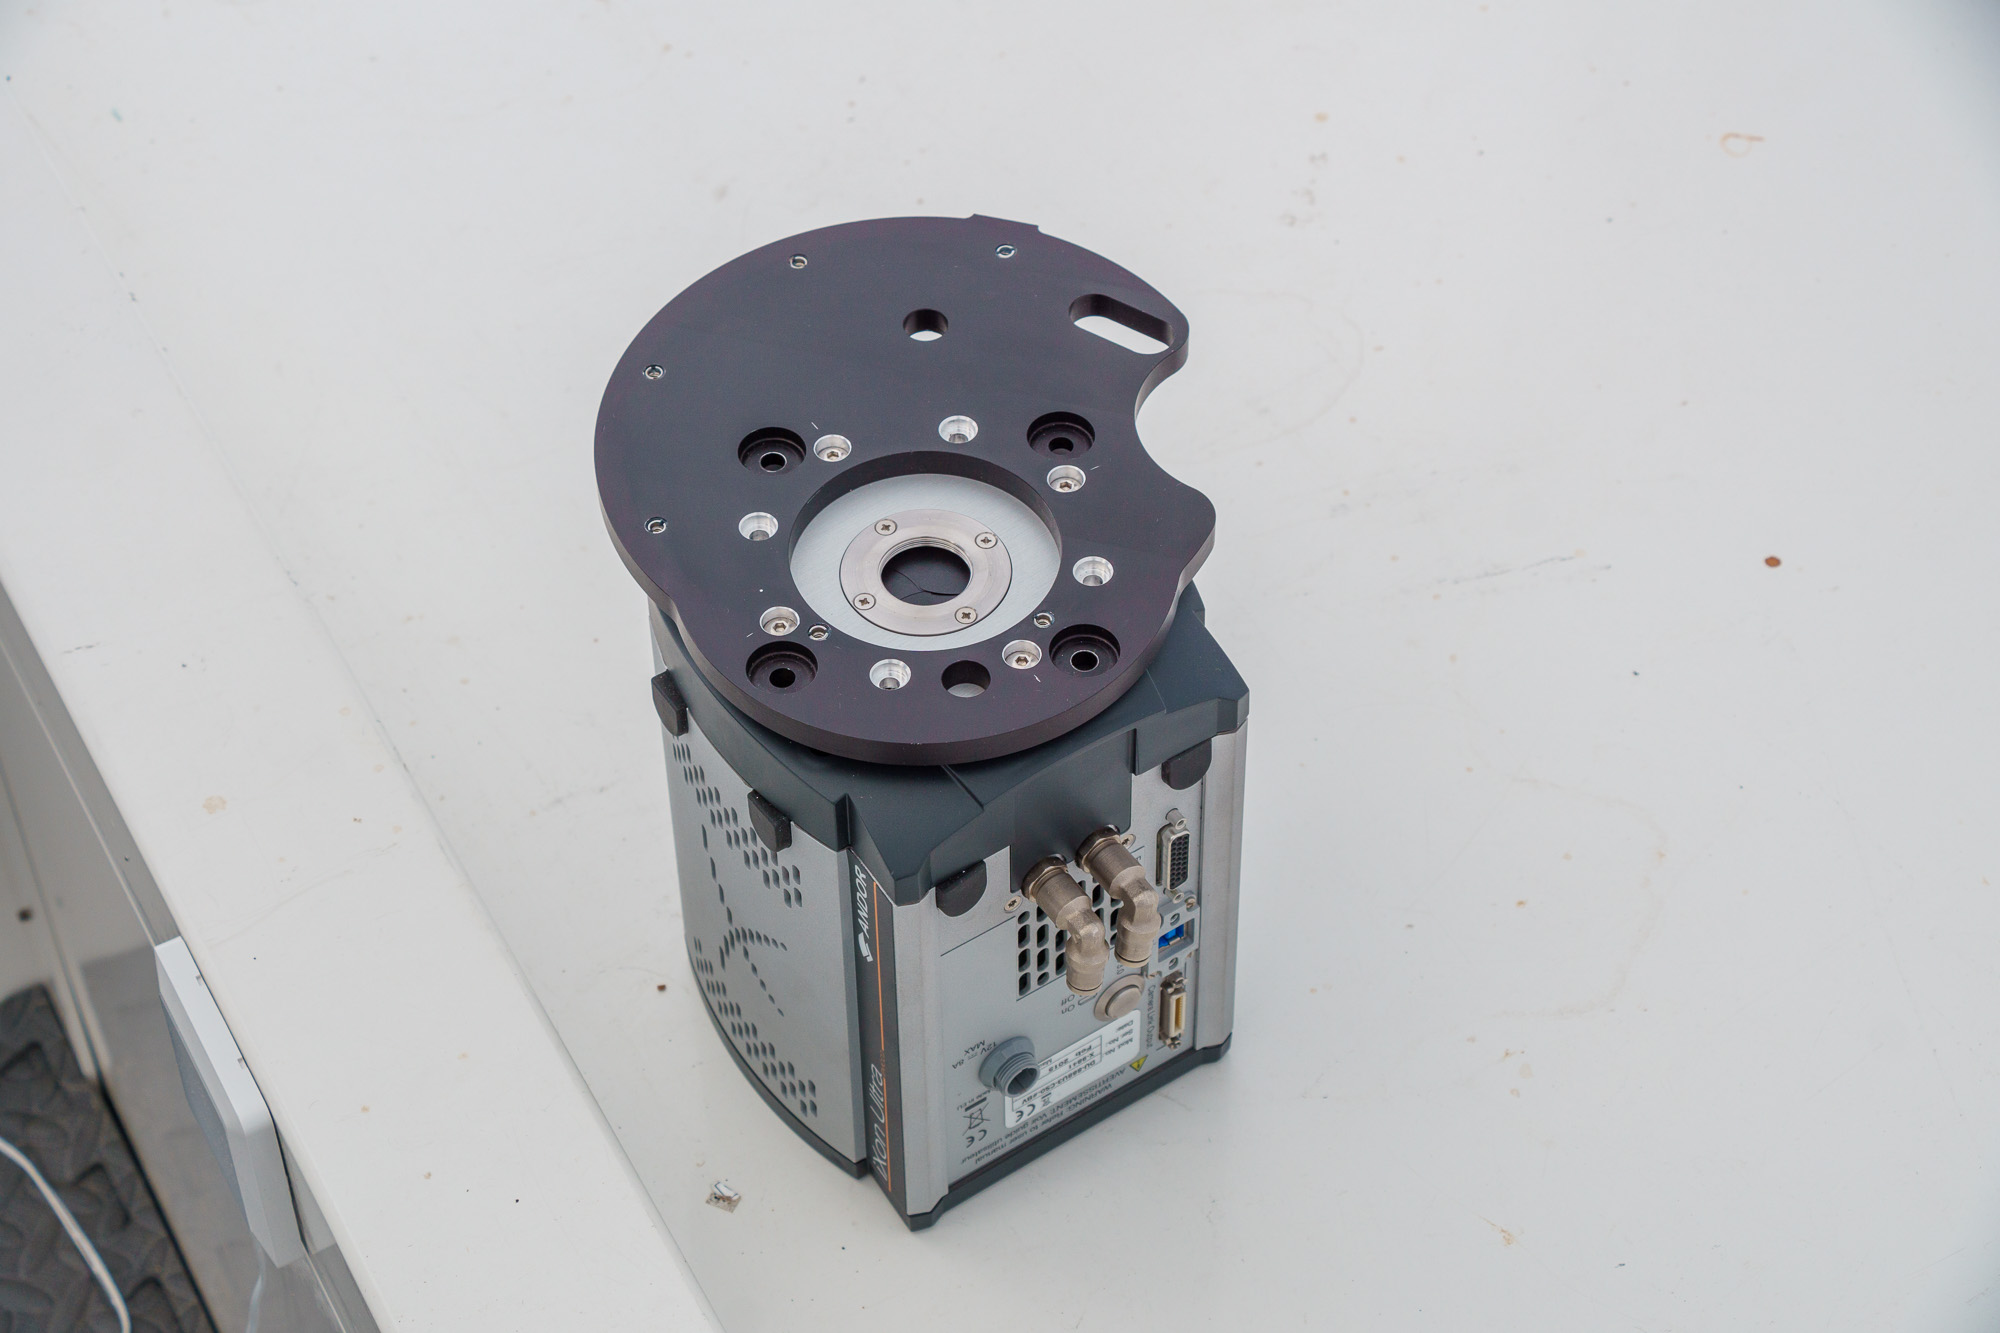
\includegraphics[width=0.8\linewidth]{figures/huitzi-without-rear-cone.jpg}
\end{center}
\caption{The detector without the rear light baffle cone. The four screws that hold the rear plate to the detector can be seen here. Note that the holes for the screws are indicated with scratched lines.}
\label{figure:huitzi-without-rear-cone}
\end{figure*}

\begin{enumerate}

    \item Go to the shed. Put on harnesses and helmets. Move the enclosure switch to LOCAL. Open the enclosure to 60 degrees. Ascend to the platform.

    \item Move the telescope to the home position (above the mount and pointed at the north pole). To do this, press the brake button and move the telescope by hand. This is important, as after the instrument is removed the telescope will not be balanced.

    \item Turn off the detector by pressing the power button on its underside. See Figure~\ref{figure:huitzi-detector-power-button}.

    \item Disconnect the four cables: detector USB and power and filter wheel USB and power (see Figure~\ref{figure:huitzi-cables-disconnected}).

    \item Dismount the filter wheel and detector by removing the six screws that hold them to the separator barrel. See Figure~\ref{figure:huitzi-mounting-screws}. Use a 4 mm hex key.  One person should support the filter wheel and detector while the other removes the screws.

    \item Place the filter wheel and detector in a safe place resting on the rear surface of the detector. The covered end of the enclosure is ideal. See Figure~\ref{figure:huitzi-off-telescope}.

    \item If you do not need to operate the instrument when dismounted, skip this step.
    
    If you do need to operate the instrument when dismounted, the easiest approach is place the instrument on the steps just to the south of the columm. Be careful that the steps do not penetrate the duct-taped gap between the column and the platform.
    Then, disconnect the Igus Triflex chain from the telescope and remove the white secondary cable. Finally, connect the detector and filter wheel cables to the instrument and press the power button on the detector. See Figure~\ref{figure:huitzi-operating-off-telescope}.
    
    \item If you do not need access to the filter wheel and/or detector, stop here.  If you do, continue.
    
    \item Remove the two set screws between the filter wheel and the detector. Use a 5/16 inch hex key. See Figure~\ref{figure:huitzi-set-screws}.
    
    \item Remove the the six screws that pass from the front plate, through the wheel, and into the rear plate. Use a 2 mm hex key. See Figure~\ref{figure:huitzi-off-telescope}.
    
    \item Remove the front plate to expose the filter wheel and spacer. See Figure~\ref{figure:huitzi-without-front-plate}.
    
    \item Remove the spacer to expose the filter wheel. See Figure~\ref{figure:huitzi-without-spacer}.
    
    \item Remove the filter wheel. See Figure~\ref{figure:huitzi-without-filter-wheel}.
    
    \item If you do not need access to the detector, stop here. If you do, continue.
    
    \item Remove the rear light baffle cone from the rear plate. It is held in place by friction.  See Figure~\ref{figure:huitzi-without-filter-wheel}. 
    
    \item Remove the four screws that hold the rear plate to the detector flange. Use a 4 mm hex key. See Figure~\ref{figure:huitzi-without-rear-cone}.

\end{enumerate}

\subsubsection{Mounting the Imager}

\begin{enumerate}

    \item Go to the shed. Put on harnesses and helmets. Move the enclosure switch to LOCAL. Open the enclosure to 60 degrees. Ascend to the platform.

    \item Replace the four screws that hold the rear plate to the detector flange. Use a 4 mm hex key. The correct holes for the screws are indicated with scratches on the rear plate. Note the orientation of the plate. See Figure~\ref{figure:huitzi-without-rear-cone}.

    \item Replace the rear light baffle cone from the rear plate.See Figure~\ref{figure:huitzi-without-filter-wheel}. 

    \item Replace the filter wheel. See Figure~\ref{figure:huitzi-without-filter-wheel}.

    \item Replace the spacer. See Figure~\ref{figure:huitzi-without-front-plate}.
    
    \item Replace the front plate. See Figure~\ref{figure:huitzi-off-telescope}.
    
    \item Replace the the six screws that pass from the front plate, through the wheel, and into the rear plate. Use a 2 mm hex key. See Figure~\ref{figure:huitzi-off-telescope}.

    \item Replace the two set screws between the filter wheel and the detector. Use a 5/16 inch hex key. See Figure~\ref{figure:huitzi-set-screws}.

    \item Mount the filter wheel and detector by replacing the six screws that hold them to the separator barrel. See Figure~\ref{figure:huitzi-mounting-screws}. Use a 4 mm hex key. One person should support the filter wheel and detector while the other replaced the screws. Note the orientation of the filter wheel and detector. The arrows scratched on the separator barrel and front plate should be aligned.

   \item Connect the four cables: detector USB and power and filter wheel USB and power (see Figure~\ref{figure:huitzi-cables-disconnected}).

   \item Turn on the detector by pressing the power button on its underside. See Figure~\ref{figure:huitzi-detector-power-button}.

\end{enumerate}

\subsection{Changing a Filter}

\subsubsection{Requirements}

You will need:

\begin{itemize}
    \item Two persons.
    \item The key to the shed.
    \item 4 mm and 2 mm hex keys (to dismount and mount the instrument).
    \item 5/16 inch hex key (to dismount and mount the instrument).
    \item A clean plastic bag to transport the filter wheel. There are bags in the COATLI/DDOTI tool cabinet.
    \item PH1 screwdriver.
    \item Tweezers
    \item Nitrile gloves
    \item If replacing a 5 mm filter with a 3 mm filter, one of the 25 mm O-rings supplied with the filter wheel.
\end{itemize}

\subsubsection{Procedure}

\begin{figure*}
\begin{center}
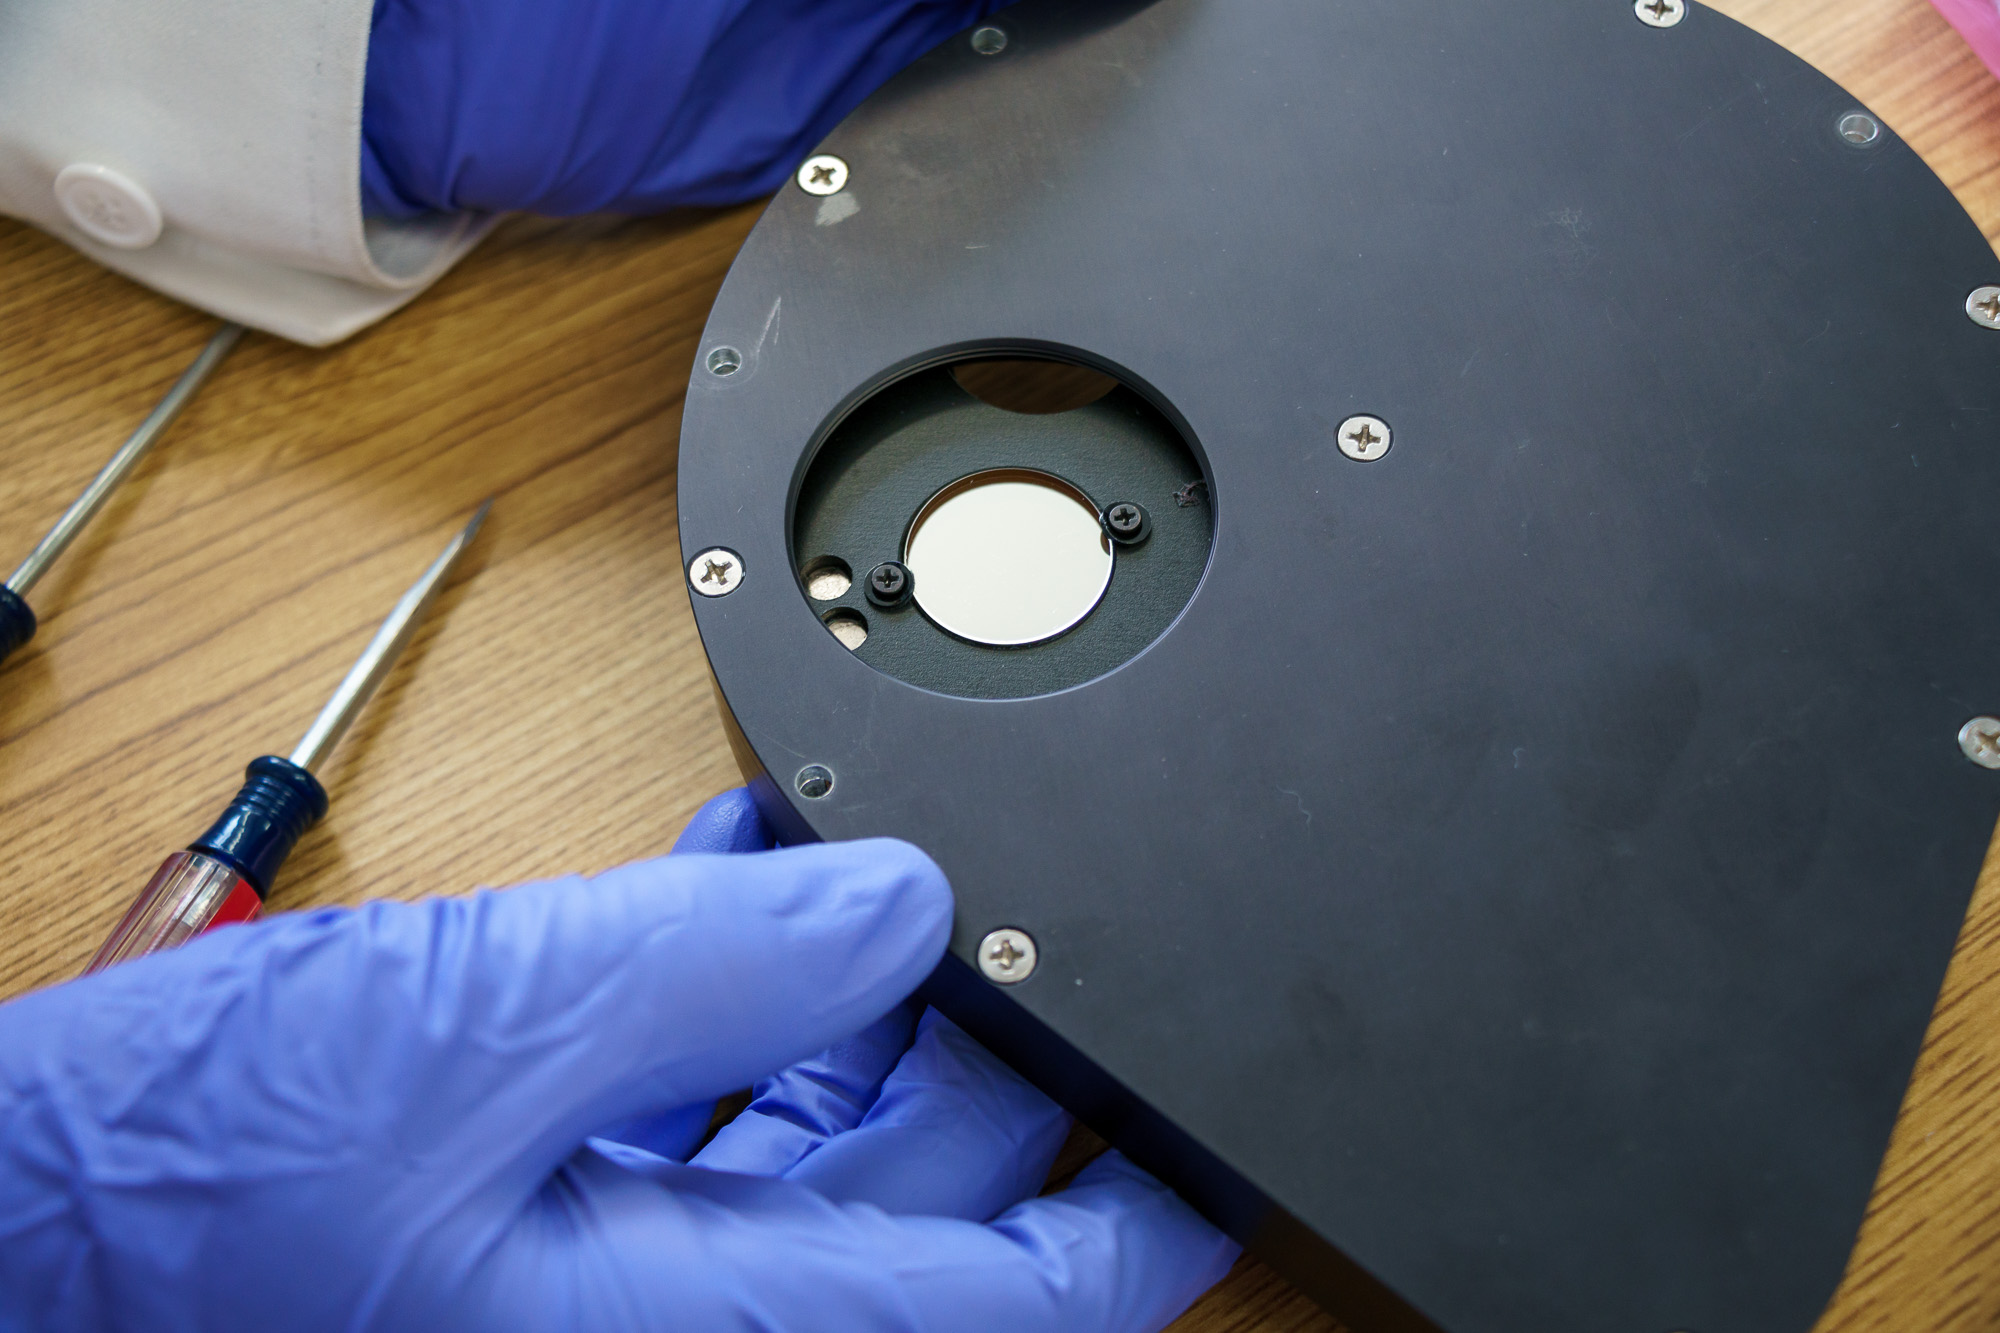
\includegraphics[width=0.8\linewidth]{figures/huitzi-filter-wheel-slots.jpg}
\end{center}
\caption{The filter wheel. There are 8 filter slots, labelled 0 to 7. The filter wheel can be moved by hand.}
\label{figure:huitzi-filter-wheel-slots}
\end{figure*}

\begin{figure*}
\begin{center}
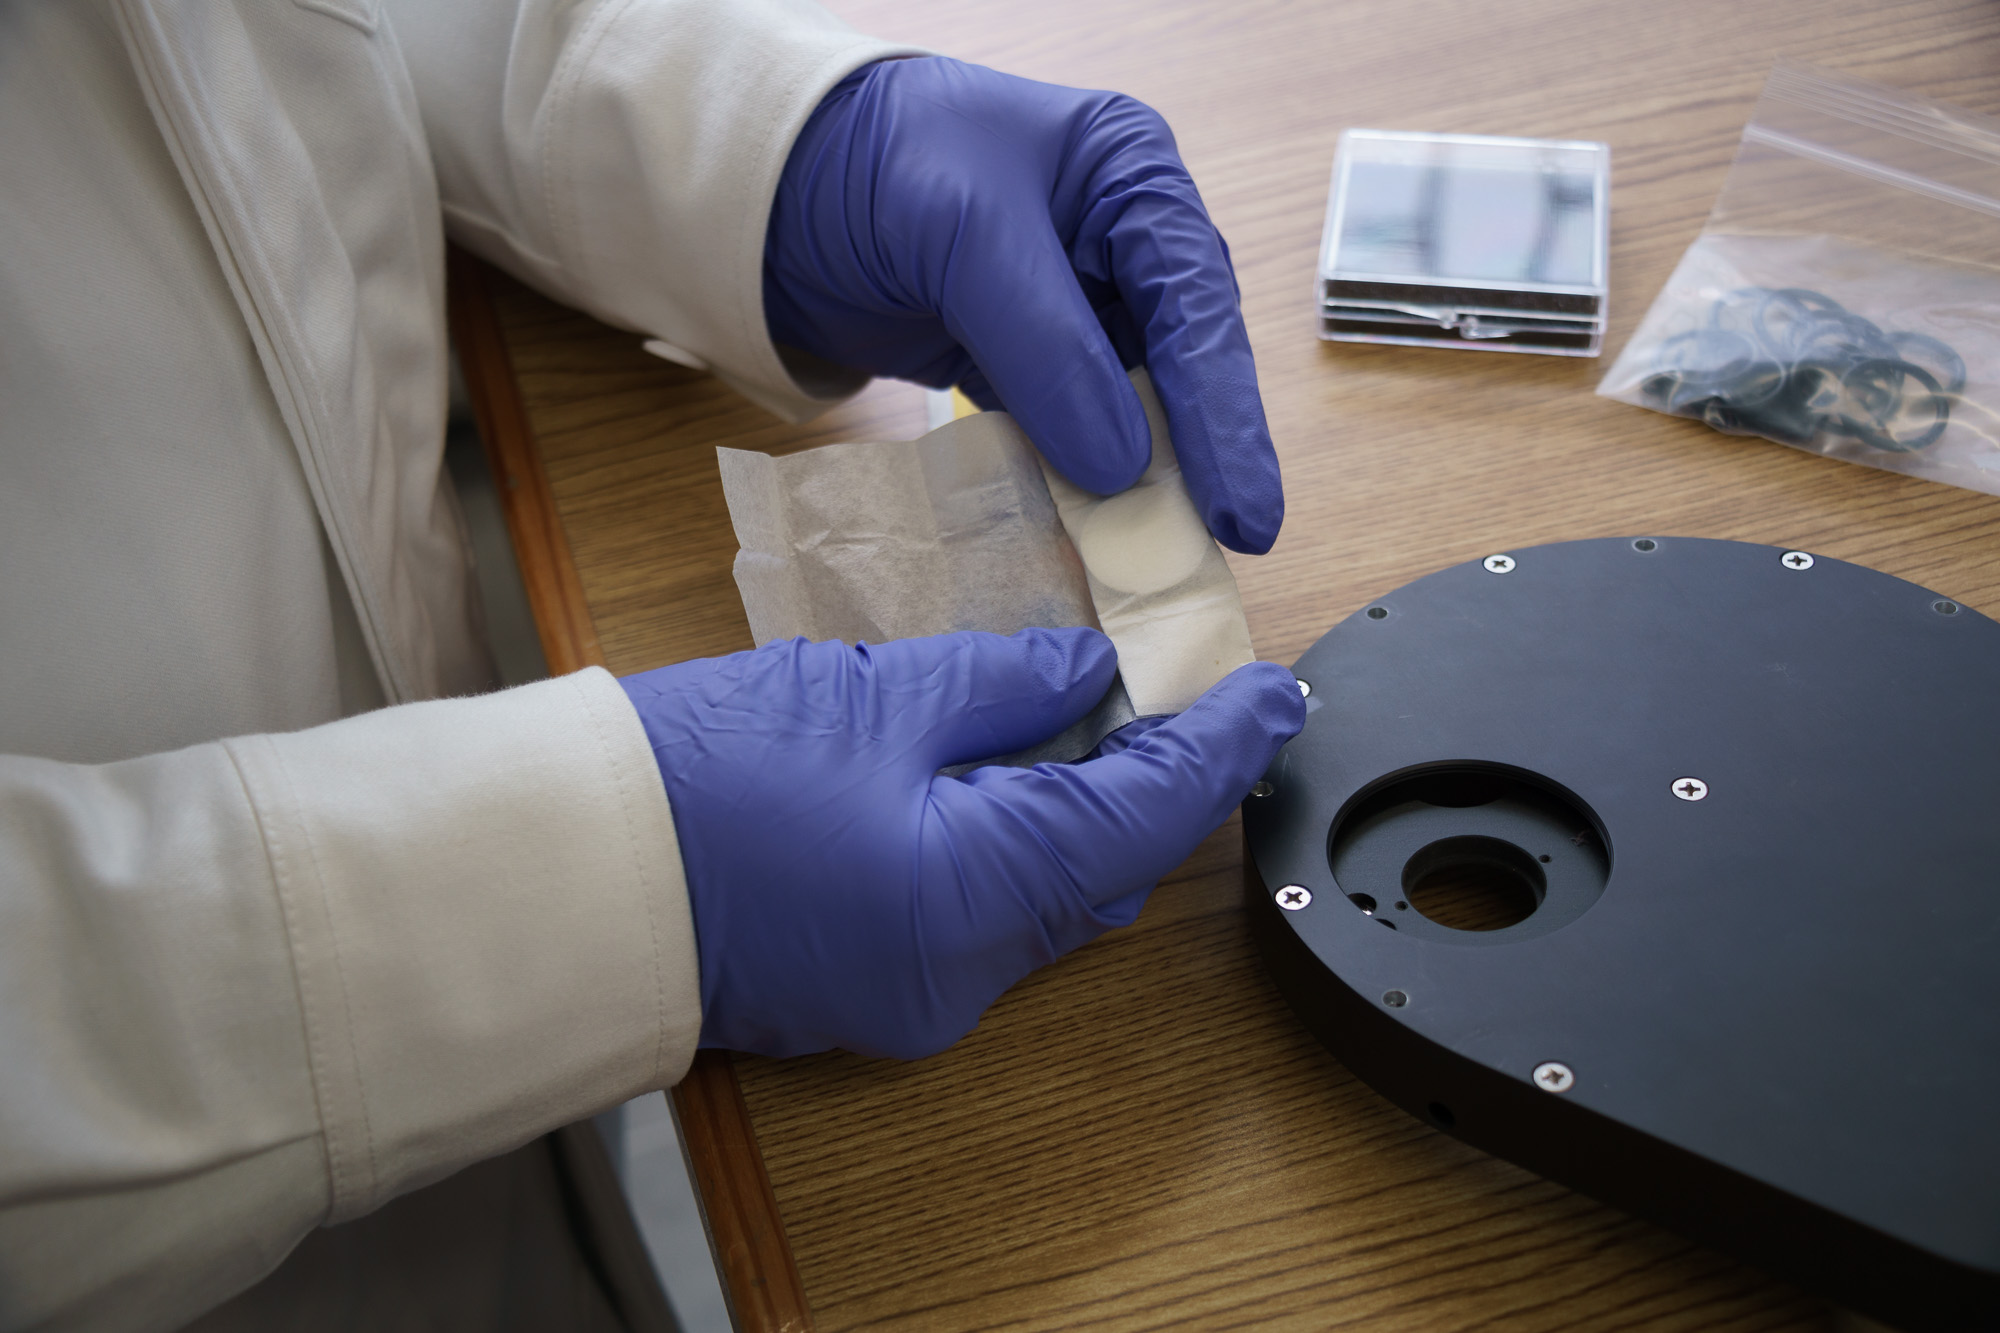
\includegraphics[width=0.8\linewidth]{figures/huitzi-filter-paper.jpg}
\end{center}
\caption{The filters are wrapped in optical paper.}
\label{figure:huitzi-filter-paper}
\end{figure*}

\begin{figure*}
\begin{center}
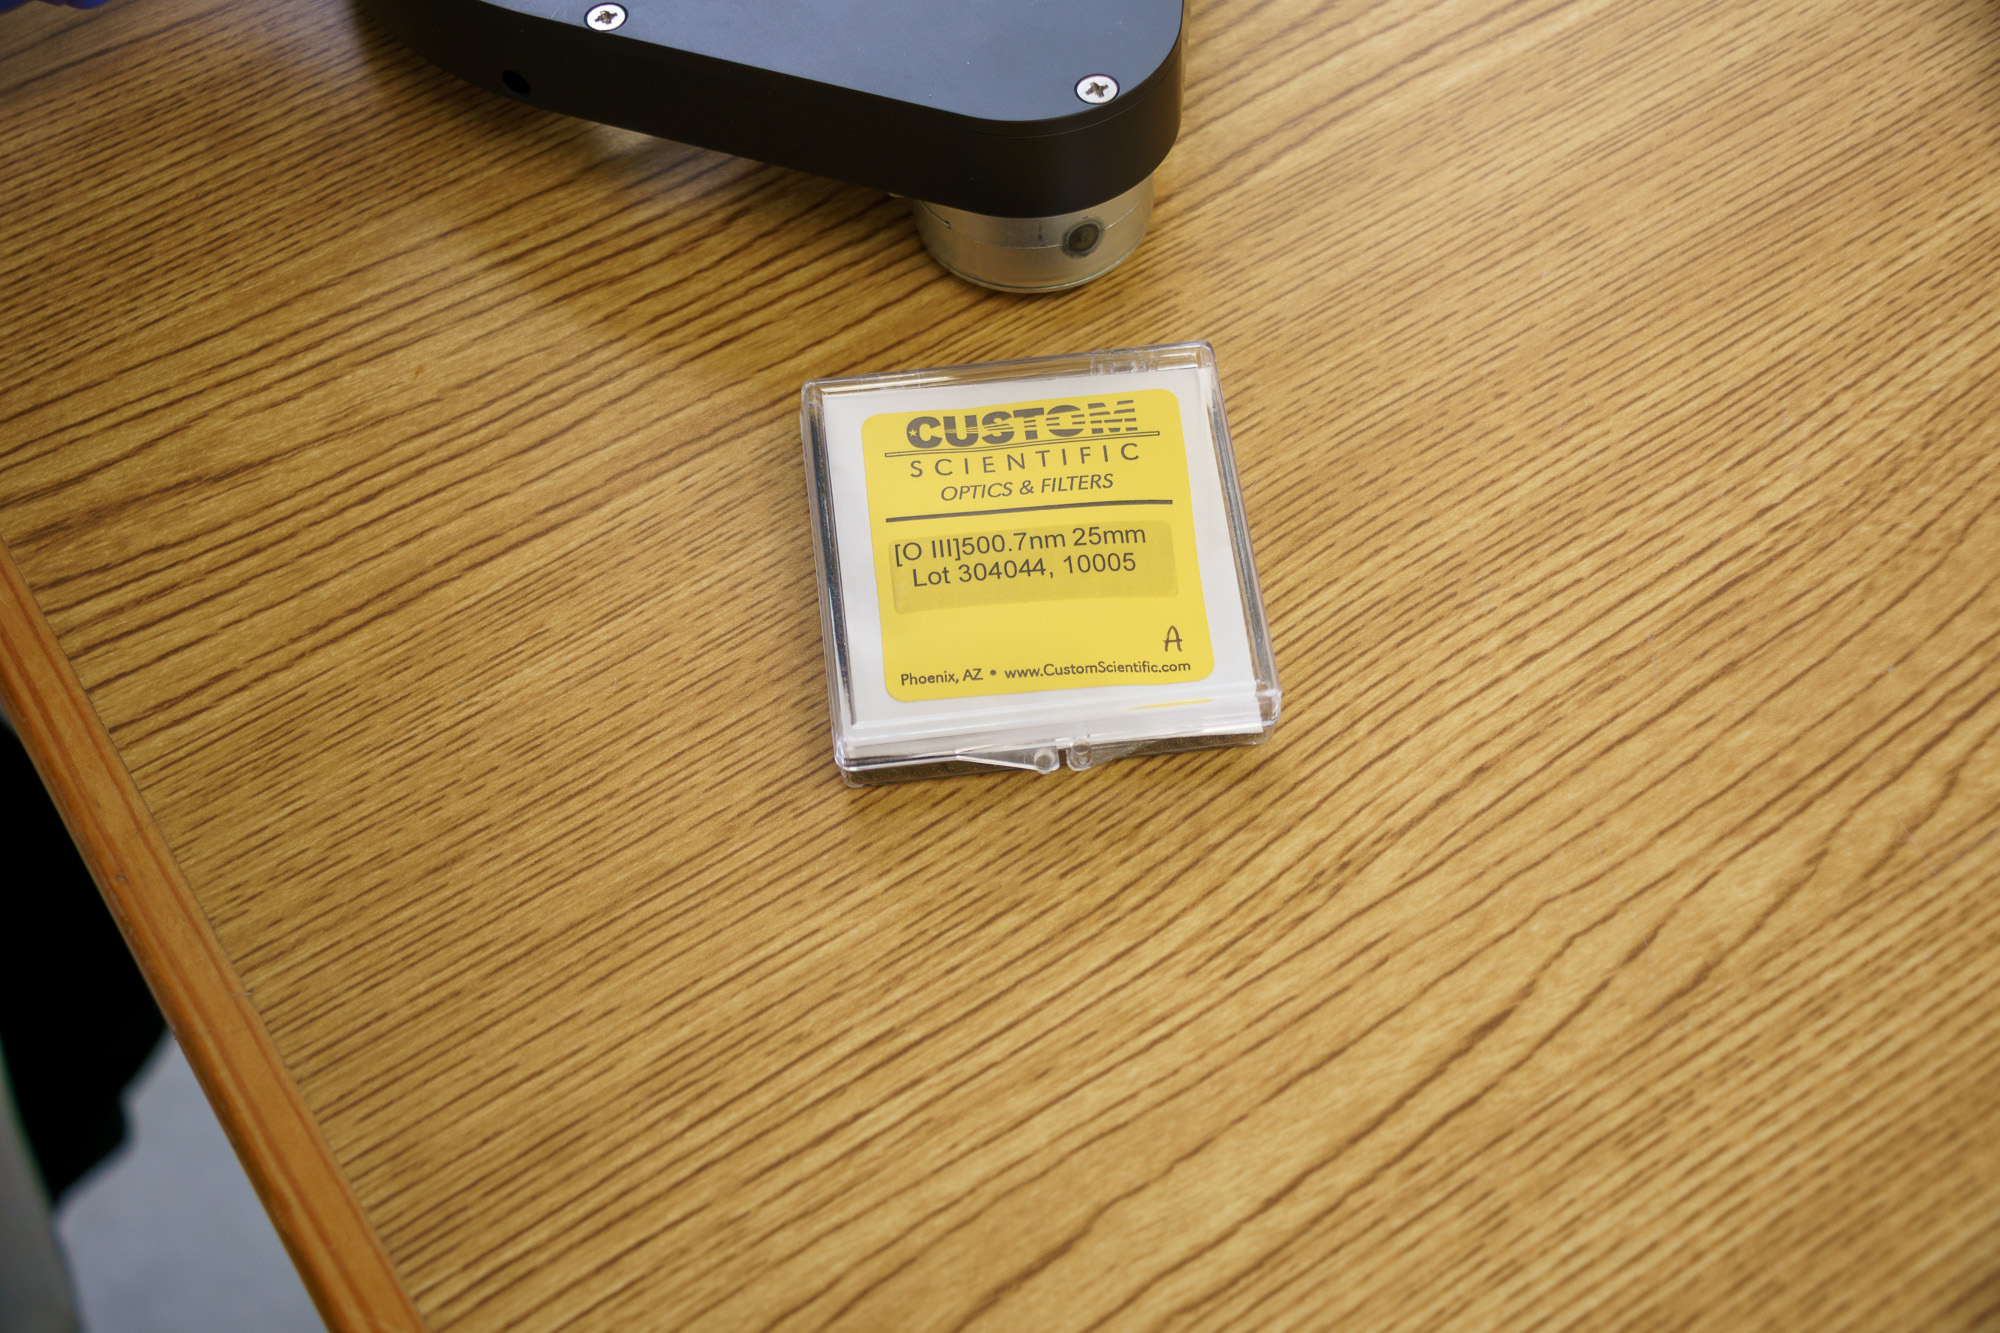
\includegraphics[width=0.8\linewidth]{figures/huitzi-filter-case.jpg}
\end{center}
\caption{The filters are protected by cases like this one.}
\label{figure:huitzi-filter-case}
\end{figure*}

\begin{figure*}
\begin{center}
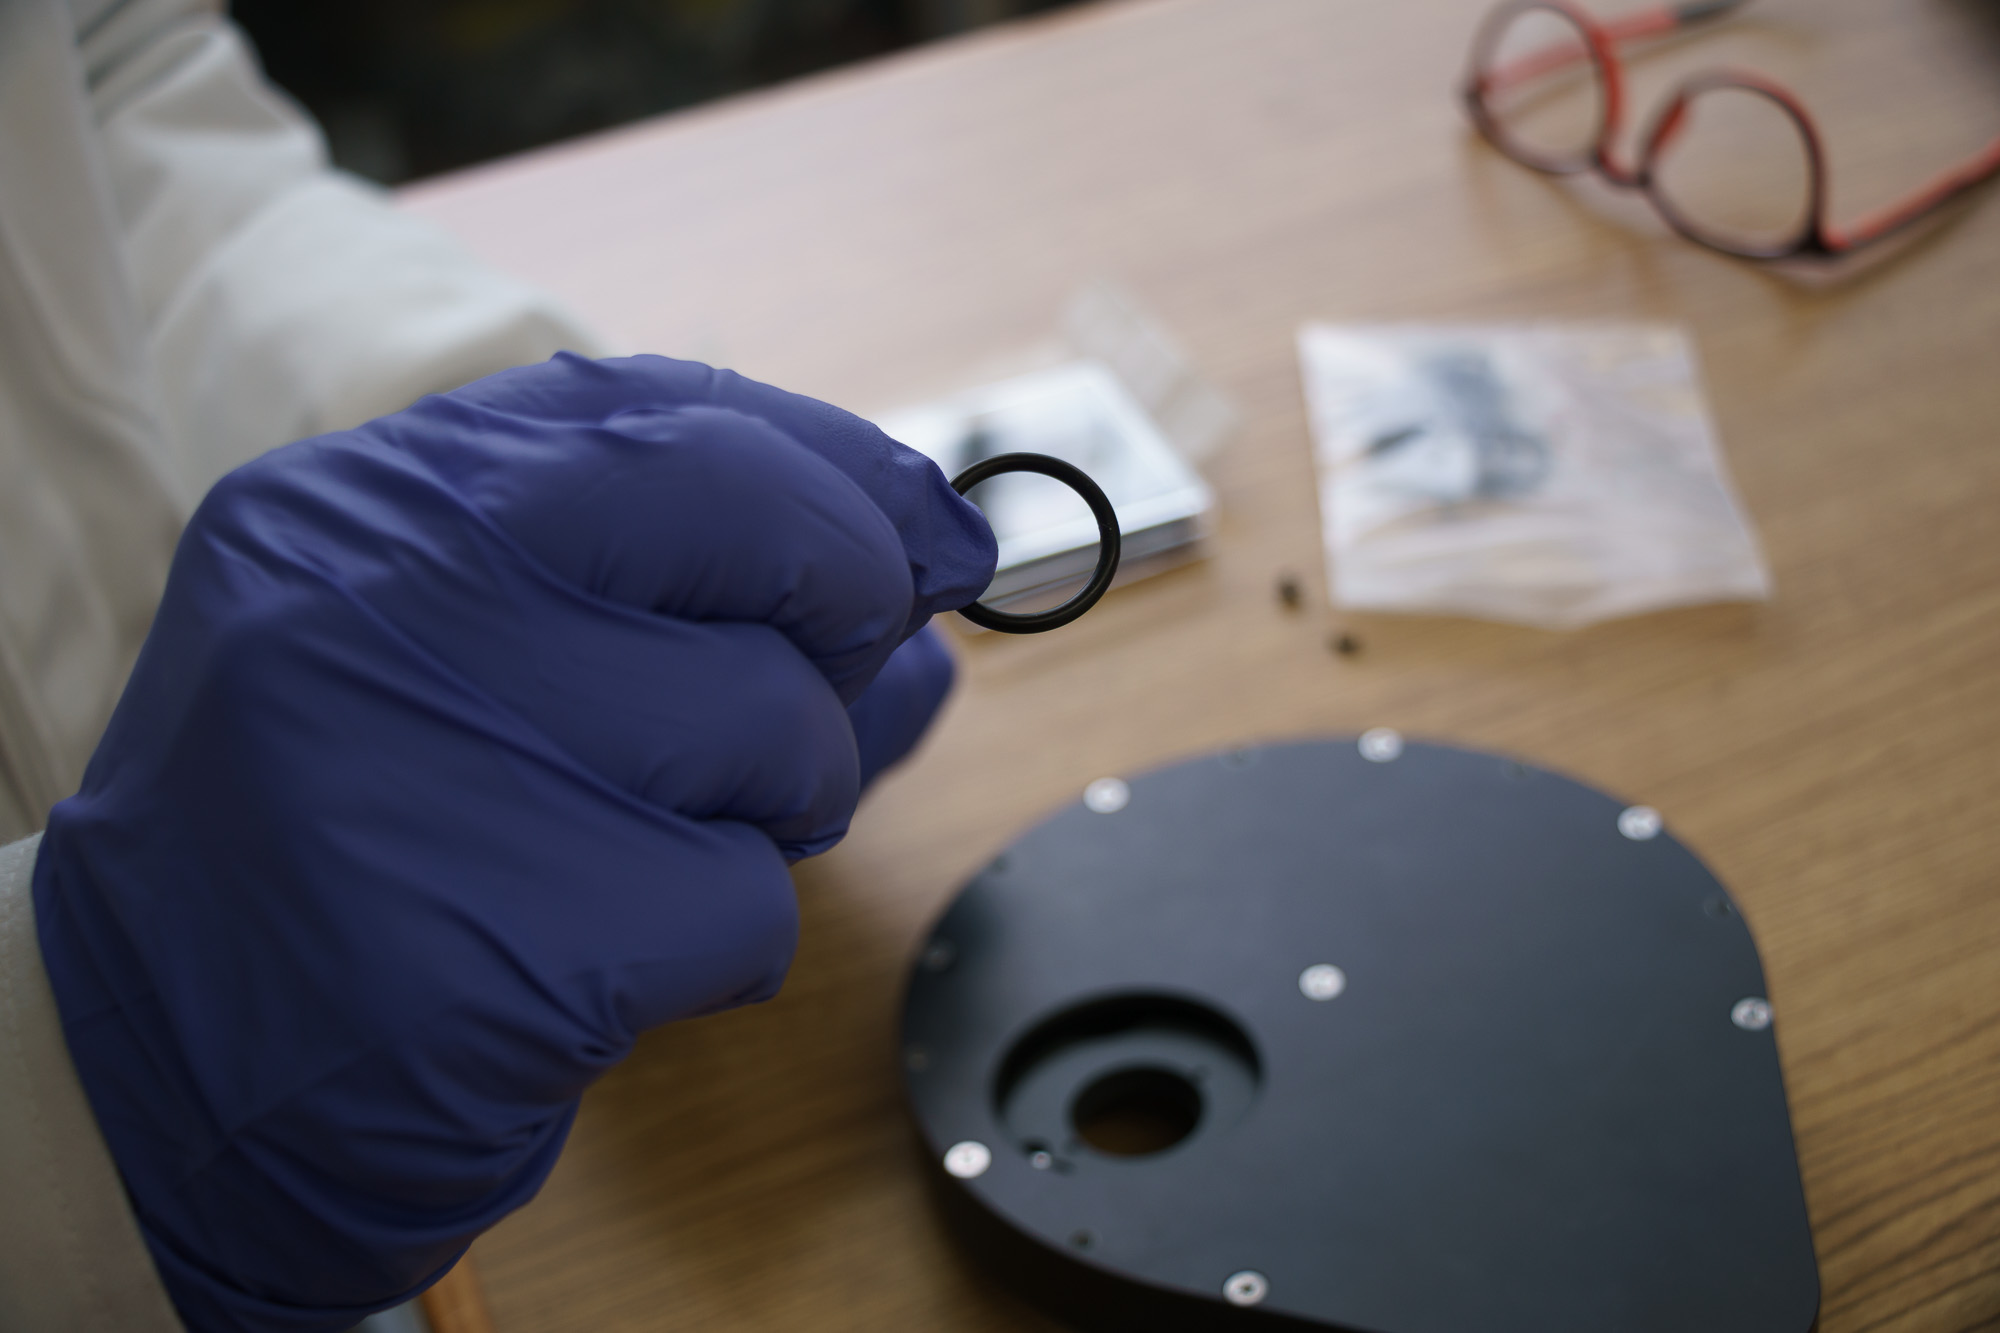
\includegraphics[width=0.6\linewidth]{figures/huitzi-filter-wheel-o-ring-a.jpg}
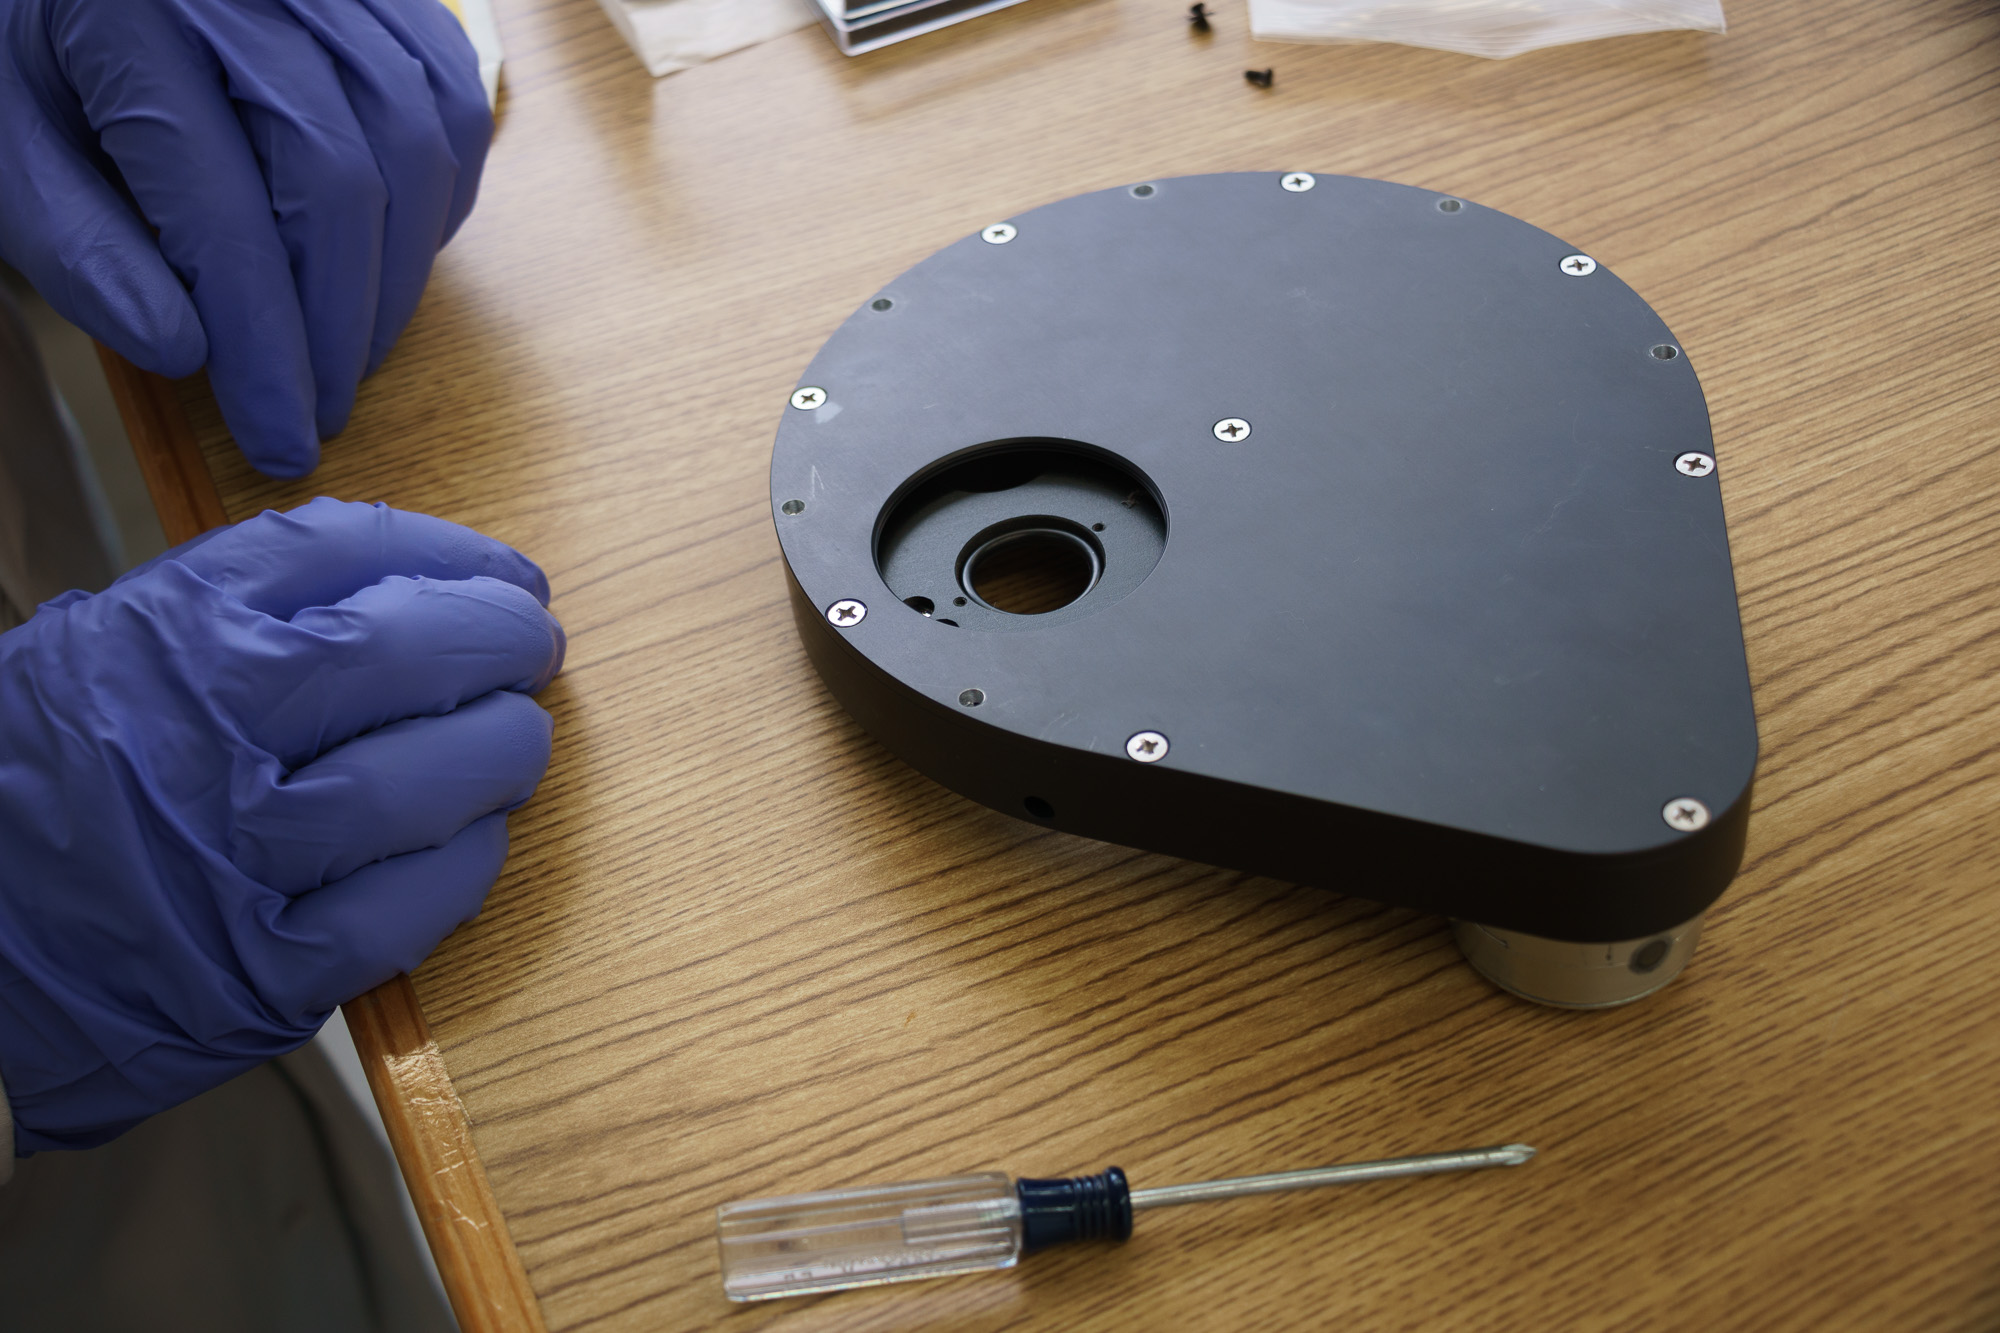
\includegraphics[width=0.6\linewidth]{figures/huitzi-filter-wheel-o-ring-b.jpg}
\end{center}
\caption{The difference in thickness between the 3 mm and 5 mm thick filters is compensated by an O-ring.}
\label{figure:huitzi-filter-wheel-o-ring}
\end{figure*}

\safety{Filters are delicate optical components. Work in the laminar-flow cabinet at the 2.1 meter. Handle them by their edges. They should only be cleaned by optical engineers.}

\safety{Do not remove dust from filters by blowing them with compressed air from a compressor, cylinder, or can, as these sources can contain oil. Only use a hand blower (perilla).}

\begin{enumerate}
    \item Remove the filter wheel from the instrument. See \S\ref{section:huitzi-dismounting-and-mounting}.
    \item Place the filter wheel in the clean plastic bag. Take the filter wheel to the optical workshop at the 2.1 meter. Replace the filters in the laminar-flow cabinet to avoid dust.
    \item Use nitrile gloves.
    \item Move the filter wheel by hand to expose the correct filter. See Figure~\ref{figure:huitzi-filter-wheel-slots}. The 8 filter slots are labelled from 0 to 7.
    \item Remove the two screws and washers that hold the filter in place. See Figure~\ref{figure:huitzi-filter-wheel-slots}.  Use the PH1 screwdriver and the tweezers.
    \item Use one finger to push the filter from below and the other hand to remove the filter.
    \item Wrap the filter in optical paper (which should be in its box). See Figure~\ref{figure:huitzi-filter-paper}.
    \item Replace the filter in its case. See Figure~\ref{figure:huitzi-filter-case}.
    \item If you are replacing a 5 mm thick filter ($griz$ and $BVRI$) with a 3 mm thick filter (the medium-band $XXX$/10 and narrow-band $XXX$/3 filters), place a 25 mm O-ring in the filter slot. See Figure~\ref{figure:huitzi-filter-wheel-o-ring}.
    
    If you are replacing a 3 mm thick filter with a 5 mm filter, remove the 25 mm O-ring from the slot and store it the ziploc bag that contains the others.
    
    \item Place the filter in the slot. For interference filters (all but $BVRI$), the bandpass coating (which will often appear to be reflective) should be on the side towards the filter wheel motor. This is down in the orientation shown in \ref{figure:huitzi-filter-wheel-slots} but up once the filter wheel is installed on the telescope.
    
    \item Replace the  two screws and washers that hold the filter in place. See Figure~\ref{figure:huitzi-filter-wheel-slots}.  Use the PH1 screwdriver and the tweezers. The washers should make contact with the filter. We find it is easiest to insert both screws first without tightening either and then tighten each in turn. You can use tweezers to make sure the washers are positioned correctly.
    
    \item If necessary, use a hand blower (perilla) to remove dust from the filter surfaces.
    
    \item Make sure the filter wheel can turn without the screws interfering with the casing. Do this by turning the filter wheel by hand.
    
    \item Place the filter wheel in the clean plastic bag. Return it to the platform.
    
    \item Replace the filter wheel in the instrument. See \S\ref{section:huitzi-dismounting-and-mounting}.

\section{Bibliography}

\begin{flushleft}
\begin{itemize}
\item “\href{bibliography/huitzi/andor-ixon-ultra-888-data-sheet.pdf}{Andor iXon Ultra 888 Data Sheet}”, Andor, May 2014.
\item “\href{bibliography/huitzi/andor-ixon-ultra-888-hardware-guide.pdf}{Andor iXon Ultra \& Life 888 Hardware Guide}”, Andor, Version 1.8 of 30 September 2019.
\item “\href{bibliography/huitzi/e2v-ccd201-20-datasheet.pdf}{CCD201-20 Datasheet}”, Teledyne e2v, Version 7 of August 2019.
\end{itemize}
\end{flushleft}
    
\end{enumerate}